\documentclass[12pt, a4paper]{memoir} % for a short document
\usepackage[french,english]{babel}

\usepackage [vscale=0.76,includehead]{geometry}                % See geometry.pdf to learn the layout options. There are lots.
%\geometry{a4paper}                   % ... or a4paper or a5paper or ...
%\geometry{landscape}                % Activate for for rotated page geometry
%\OnehalfSpacing
% \setSingleSpace{1.05}
%\usepackage[parfill]{parskip}    % Activate to begin paragraphs with an empty line rather than an indent
\usepackage{graphicx}
\usepackage{amsmath,amssymb}
\usepackage{amsfonts}
\usepackage{amsthm}
\usepackage{bbm}
\usepackage{fullpage}
\usepackage{mathptmx} % font = times
\usepackage{helvet} % font sf = helvetica
\usepackage[T1]{fontenc}
\usepackage[utf8]{inputenc}
\usepackage{relsize}
\usepackage{float}
\usepackage{accents}
\usepackage{caption}
\usepackage{subcaption}
\usepackage[all]{xy} % for diagrams
\usepackage{listings} % for code excerpts
\usepackage{multirow} % for multicolumn / multirow arrays

\usepackage{lineno}
% \linenumbers

% Clickable links in the toc
\usepackage{hyperref}
\hypersetup{
    colorlinks,
    citecolor=black,
    filecolor=black,
    linkcolor=black,
    urlcolor=black
}

% Custom commands
\newcommand{\ocirc}[1]{\accentset{\circ}{#1}}
\newcommand{\R}{\mathbb{R}}
\newcommand{\partiald}[2]{\frac{\partial{#1}}{\partial{#2}}}
\newcommand{\indicator}[1]{\mathbbm{1}_{#1}}
\newcommand{\cloud}{P}
\newcommand{\surface}{S}
\newcommand{\mean}[1]{H_{#1}}
\newcommand{\meanv}[1]{\vec{H}_{#1}}
\newcommand{\appendixref}[1]{\textit{\nameref{#1}}}

% Custom theorems
\newtheorem{definition}{Definition}
\newtheorem{proposition}{Proposition}
\newtheorem{lemma}{Lemma}
\newtheorem{theorem}{Theorem}

% Graphics path
\graphicspath{{img/}}

% Custom styles
\headstyles{komalike}
\nouppercaseheads
\chapterstyle{dash}
\makeevenhead{headings}{\sffamily\thepage}{}{\sffamily\leftmark}
\makeoddhead{headings}{\sffamily\rightmark}{}{\sffamily\thepage}
\makeoddfoot{plain}{}{}{} % Pages chapitre.
\makeheadrule{headings}{\textwidth}{\normalrulethickness}
%\renewcommand{\leftmark}{\thechapter ---}
\renewcommand{\chaptername}{\relax}
\renewcommand{\chaptitlefont}{ \sffamily\bfseries \LARGE}
\renewcommand{\chapnumfont}{ \sffamily\bfseries \LARGE}
\setsecnumdepth{subsection}

% Title page formatting -- do not change!
\pretitle{\HUGE\sffamily \bfseries\begin{center}}
\posttitle{\end{center}}
\preauthor{\LARGE  \sffamily \bfseries\begin{center}}
\postauthor{\par\end{center}}

\newcommand{\jury}[1]{%
\gdef\juryB{#1}}
\newcommand{\juryB}{}
\newcommand{\session}[1]{%
\gdef\sessionB{#1}}
\newcommand{\sessionB}{}
\newcommand{\option}[1]{%
\gdef\optionB{#1}}
\newcommand{\optionB}{}

\renewcommand{\maketitlehookd}{%
\vfill{}  \large\par\noindent
\begin{center}\juryB \bigskip\sessionB\end{center}
\vspace{-1.5cm}}
\renewcommand{\maketitlehooka}{%
\vspace{-1.5cm}\noindent
\includegraphics[height=14ex]{logoINP.png}\hfill\raisebox{2ex}{
\includegraphics[height=7ex]{logoUJF.jpg}}\\
\bigskip
\begin{center} \large
Master of Science in Informatics at Grenoble \\
Master Math\'ematiques Informatique - sp\'ecialit\'e Informatique \\
option \optionB  \end{center}\vfill}
% End of title page formatting

\option{$GVR$}
\title{Adaptive point cloud denoising}%\\\vspace{-1ex}\rule{10ex}{0.5pt} \\sub-title}
\author{Jocelyn MEYRON}
\date{26th June 2015} % Delete this line to display the current date
\jury{
Research project performed at GIPSA-lab \\\medskip
Under the supervision of:\\
ATTALI Dominique, GIPSA-lab\\
MÉRIGOT Quentin, CEREMADE, Université Paris-Dauphine\\\medskip
Defended before a jury composed of:\\
Mr CROWLEY James\\
Mr BOYER Edmond\\
Mr VAUFREYDAZ Dominique\\
Mr FRANCO Jean-Sébastien\\
Mr HÉTROY-WHEELER Franck\\
% $[$Prof/Dr/Mrs/Mr$]$ $<$first-name last-name$>$\\
}
\session{$June$\hfill 2015}

\begin{document}

% Title page
\selectlanguage{english}
\frontmatter
\begin{titlingpage}
\maketitle
\end{titlingpage}
\setlength{\parskip}{-1pt plus 1pt}

% Abstract
\renewcommand{\abstracttextfont}{\normalfont}
\abstractintoc

% English
\begin{abstract}

% TODO
During this internship, we were interested in the denoising / smoothing of point
clouds and more specifically in an adaptive one: the magnitude of the smoothing
will be more important in some privileged directions. In order to do that, we
will use a mean curvature flow based method: the idea is to move the point cloud
while minimizing an energy. This energy will be related to the Minkowski sum of
the point cloud with a convex polyhedron. The choice of this polyhedron will
determine the privileged directions of the smoothing.

This report is divided as follows: firstly, we will give a detailed introduction
on the mean curvature flow and we will prove some properties (valid in any dimension
$d$) which will be used throughout the rest of the report like the convergence
of the gradient of the energy towards the mean curvature vector.

Secondly, we will study the two dimensional case with the $r$-offset
of a point cloud. We will prove that this technique can be used to simulate a
discrete mean curvature flow. Many examples will be studied.

We will continue by looking at the 3D case where we will study the Minkowski sum
of a 3D point cloud with a convex polyhedron. Several theoretical and practical
issues will arise. We will deal with these issues and explain the choices that
were made.

\end{abstract}

\newpage
\abstractintoc
\renewcommand\abstractname{R\'{e}sum\'{e}}

% Français
\begin{abstract} \selectlanguage{french}

% TODO
Durant ce stage, nous nous sommes intéressés au débruitage / lissage de nuage de
points et plus précisément à un lissage adaptatif: le lissage sera plus
important dans certaines directions privilégiées. Les techniques utilisées
seront basées sur le flot de courbure moyenne: l'idée est de faire évoluer le
nuage de points tout en minimisant une énergie. Cette dernière sera liée à la
somme de Minkowski du nuage de points avec un polyèdre convexe. Le choix de ce
polyèdre déterminera les directions privilégiées du lissage.

Ce rapport est structuré de la manière suivante: tout d'abord, nous donnerons
une introduction détaillée sur le flot de courbure moyenne et nous démontrerons
des propriétés (valable en dimension quelconque) que nous utiliserons tout au
long du rapport comme la convergence du gradient de l'énergie considérée vers le
vecteur courbure moyenne.

Ensuite, nous étudierons le cas bidimensionnelle en choisissant le $r$-offset
d'un nuage de points. Nous montrerons que cette technique peut être utilisée
pour simuler un flot de courbure moyenne discret. Beaucoup d'exemples
illustreront ces résultats.

Par la suite, nous nous intéresserons au cas 3D pour lequel nous étudierons la
somme de Minkowski d'un nuage de points avec un polyèdre convexe. Nous serons
confrontés à des difficultés aussi bien théoriques que pratiques. Nous
expliquerons alors les choix qui ont été faits pour résoudre les problèmes
rencontrés.

\end{abstract}

\selectlanguage{english}

% vim: set spelllang=en :

\cleardoublepage

\tableofcontents* % the asterisk means that the table of contents itself isn't put into the ToC
\normalsize

\mainmatter
\SingleSpace

% Main matter
% partie logiciel:
% 2D

% 3D 1: intersection de demi-espaces -> associer plane + inter pour AD (lien avec AD), type de nombre
% 3D 2: inclusion-exclusion
% -> environ 3 pages + bouts de codes

\chapter{Introduction}

Point clouds are useful objects in all the domains related to computer-based
processing like image processing or computer graphics because they can
represent any 3D object by only storing coordinates of points on this object. We
can obtain them from, for example, digitizing device such as a 3D scanner. A 3D
scanner is a tool which can scan a real 3D object, a surface, using for example
lasers. It samples points on the object to obtain a numeric version of the
scanned object. They can be then used to create more complex and complete models
like meshes which can be used in a software. For example, we can use surface
reconstruction algorithms like \cite{alexa2003computing}. But an important
problem arises from this technique: since the 3D scanner is a physics-based
tool, error will be made during the measurement: the resulting point cloud will
be noisy. We will be interested in removing this noise from the point cloud: we
call this technique denoising or smoothing.

There is also an other issue: we only deal with points and so we can not use all
the techniques developed in image processing like the Fourier transform,
wavelets... This is because, when we have an image, we can parametrize it
easily, for example, as a grid of pixels.  When we have a mesh, we have a kind
of parametrization but when we have only points, we do not have such
parametrization.

Several ways already exist to remove this noise and so to smooth point clouds.
Some are based on Computer Vision algorithms and some are more Computational
Geometry-based.

\begin{itemize}
    \item \textit{Gaussian / Laplacian smoothing}: replace a vertex by an other point
        computed along the nearest neighbours of the vertex. For the Laplacian
        case, the new point is the average of the neighbours (see
        \cite{vollmer1999improved}).
    \item \textit{Jet fitting} (see \cite{cazals2005estimating}): a jet is a truncated
        Taylor expansion. Such jets are fitted around points. Jet smoothing
        operates by projecting the input points on an estimated smooth
        parametric surface (the so-called jet surface). Jets are good because
        they intrinsically contain differential information such as normal,
        curvature...
    \item \textit{Bilateral smoothing} (see \cite{huang2013edge}): it is a way to do a
        smoothing while taking account the sharp edges present in the point set.
\end{itemize}

During this internship, we will use the following idea: move each point in the
direction of the inward normal by a quantity related to the mean curvature at
that point. The more curved is the surface, the more important the displacement
will be. The evolution of the surface can be modelled using a partial
differential equation. We will obtain a family of surfaces indexed by the time,
this family is called the mean curvature flow (MCF) of the initial surface.

The MCF can be seen as the geometric equivalent of the heat equation: indeed,
the Laplacian is replaced by the mean curvature vector. Both of them are sums of
eigenvalues of some matrices: the Hessian for the first one and the Shape
operator for the second.

% TODO: heat

The MCF is well-known for its smoothing properties (see
\cite{ciomaga2010level}). For example, the figure
\ref{fig:mean-curvature-flow-ex} is an illustration of the mean curvature flow
on a noised surface (extracted from \cite{clarenz2000anisotropic}).

\begin{figure}[h]
    \centering
    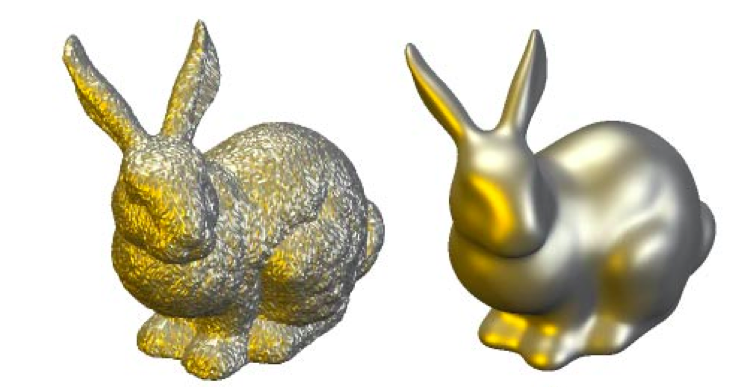
\includegraphics[scale=0.3]{img/mean-curvature-flow-rabbit}
    \caption{Mean curvature flow on a noised surface}
    \label{fig:mean-curvature-flow-ex}
\end{figure}

We will show in the last chapter of this report that this flow is linked to the
variation of the area of the surface. If we try to transform the surface while
minimizing the area, we will obtain the same evolution as the one given by the
MCF. But let us recall that we only know points sampled on a surface and not the
underlying surface. So, we will need a way to compute the area without knowing
the original surface. A common way of doing it is to consider the volume of the
union of balls centered on the points of the cloud.  We will show that this
quantity is proportional, under some sampling conditions, to the area of the
underlying surface.

Now that we have our energy, we need to minimize it. Let us denote the energy by
$ E(P) $ where $ P = \{ p_1, \ldots, p_N \} $ is a point cloud. If we are in
three dimensions then we can see the energy $ E $ as a function $ E : \R^{3N}
\to \R $. The main technique used for minimizing a function are based on the
computation of the gradient of the said function, so, we will need a way to
compute the gradient of $ E $. There are multiple possibilities of doing it:
using exact formulae if they exist, using finite differences...

In this report, we will use an original technique called \textit{Automatic
    Differentiation}. This technique is described in more details in the
appendix \ref{appendix:ad}. In short, it is a technique allowing us to compute
the derivatives of any computer program. It exploits the fact that any program
can be thought as a sequence of basic arithmetic operations and elementary
functions. Now, using the chain rule and number type overloading we can compute
derivatives of any order without changing too much the cost of the original
function.  This will allow us to only take care of the computation of $ E(P) $
and not its gradient. This will also allow us to consider different kind of
energies: the volume of the union of balls, the area of the boundary of the
union and also anisotropic ones. Let us detail the latter point.

% TODO

Anisotropic smoothing is a type of smoothing where the magnitude will depend on
the point and the topology of its neighbourhood. In image processing, this
technique is called anisotropic diffusion (see \cite{weickert1998anisotropic}):
reduce the image noise without removing significant parts of the image such as
edges, lines...

During this internship, we were interested in a kind of anisotropic evolution
based on \cite{chambolle2012nonlocal} where the smoothing is adapting in
function of the direction: smoothing will be different in some privileged
directions. These directions will be given by the user.

Anisotropic flow will have applications, for example, in physics based
simulations like crystal growth simulation.  An other example would be when we
build a 3D scan of an object: we want to be able to smooth the point cloud while
preserving certain details (the signature of the author for example).

This report is structured as follows: first, we will be interested in the two
dimensional case where we will show that our discrete MCF is able to smooth a
point cloud and can be used to estimate the mean curvature vector. Then, we will
look at the 3D case where we will study the anisotropic flow. The final part
will be dedicated to the theory: we will show that the constructed discrete MCF
is effectively an approximation of the continuous MCF.

% vim: set spelllang=en :


\chapter{2D case}

% {{{1 PROBLEM
\section{Problem}

In this part, we will focus on point clouds in 2D which sample a planar curve.
We will develop algorithms to smooth them by minimizing different energies. First, we
will consider the area of a union of disks centered on the point cloud.  We will
also test other types of energies such as the perimeter of the boundary,
weighted area and weighted perimeter of the boundary.

Firstly, we will show how to compute the area of a union of disks.  Then, we
will run different experiments to verify that the gradient of a union of disks
is proportional to the mean curvature of the underlying curve. Finally, we will
run our flows on different point clouds with different parameters to show
that it can simulate discrete mean curvature flows.

% {{{1 AREA OF A UNION OF BALLS
\section{Area of a union of balls}

Let $ P $ be a finite set of points in 2D.  We call the union of disks with
radius $ r $ centered on $ P $, the $r$-offset and we will denote it by $ P^r $.

We will first need the definition of the Voronoi diagram of set of points:

\begin{definition}
    Given a set of points $ P \in \R^2 $, we define the Voronoi cell of $ p \in
    P $ by:
    $$ V(p, P) = \{ q \in E,~ \forall p' \in P,~|| p  - q || \leq || p' -
    q || \} $$
    In other words, the Voronoi cell of $ p $ is composed of all the points which are
    closer to $ p $ than to any other points in $ P $.

    Then, the Voronoi diagram of $ P $ is composed of all the Voronoi cells of $
    p \in P $. It defines a partition of the plane $ \R^2 $.
\end{definition}

For example, the figure \ref{fig:voronoi-diagram-2d} is an example of a Voronoi
diagram.

\begin{figure}[h]
    \centering
    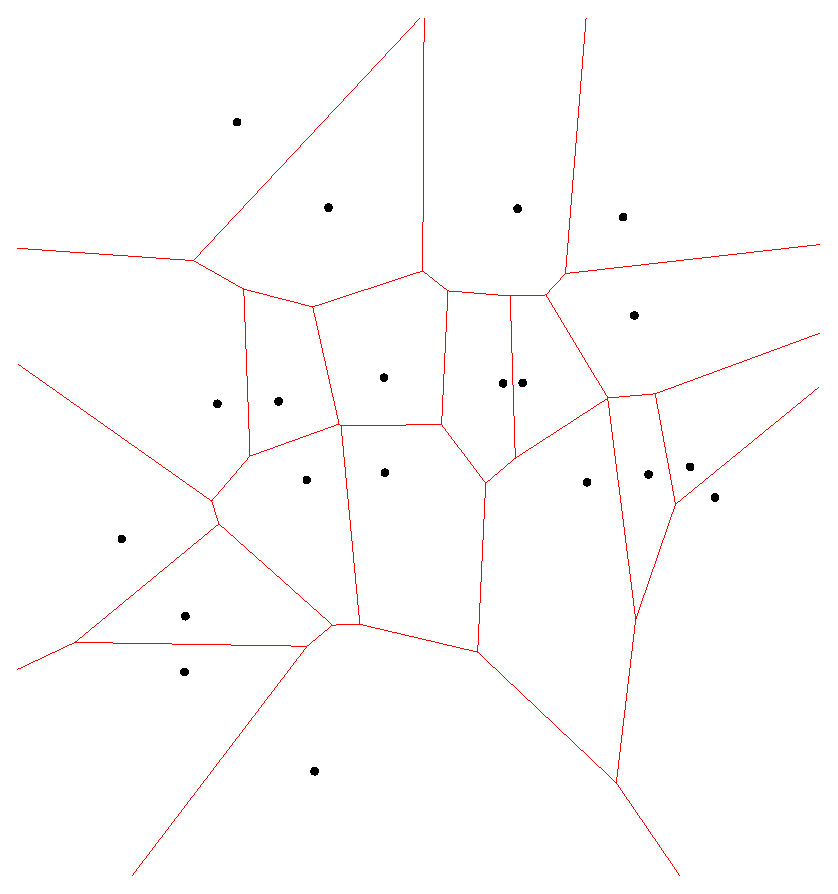
\includegraphics[scale=0.4]{voronoi-diagram-2d}
    \caption{Points are in black and the boundary of the Voronoi cells are in
        red}
    \label{fig:voronoi-diagram-2d}
\end{figure}

Now, we can say that, because the Voronoi diagram defines a partition, we have:

$$ Area(P^r) = Area \left( \bigcup_p B(p, r) \right) = \sum_p Area(V(p, P) \cap B(p, r)) $$

% {{{3 ALGORITHM
\paragraph{Algorithm}

In order to compute this quantity, we need to know how to estimate the area of the
intersection of a ball and a Voronoi cell.

The figures \ref{fig:inter_voronoi_ball_2d} illustrate the different cases for
the intersection of a Voronoi cell and a ball in 2D.

\begin{figure}[h]
    \centering
    \begin{minipage}{0.32\linewidth}
        \centering
        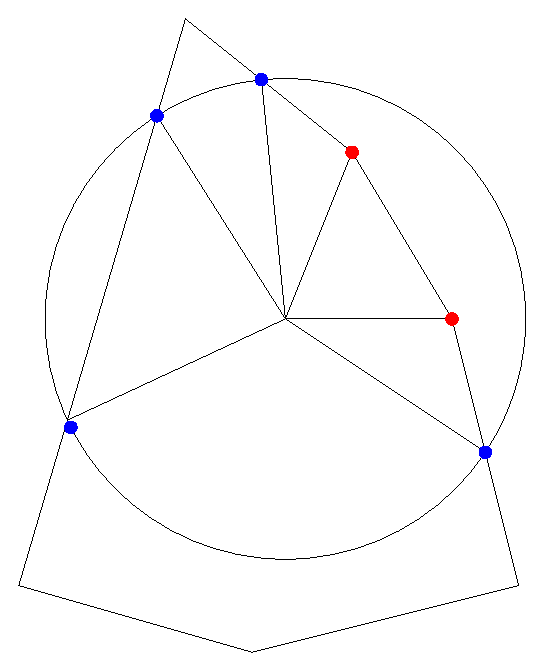
\includegraphics[scale=0.4]{2d/inter_voronoi_ball_2d}
        \subcaption{General case}
        \label{fig:inter_voronoi_ball_2d:a}
    \end{minipage}
    \begin{minipage}{0.32\linewidth}
        \centering
        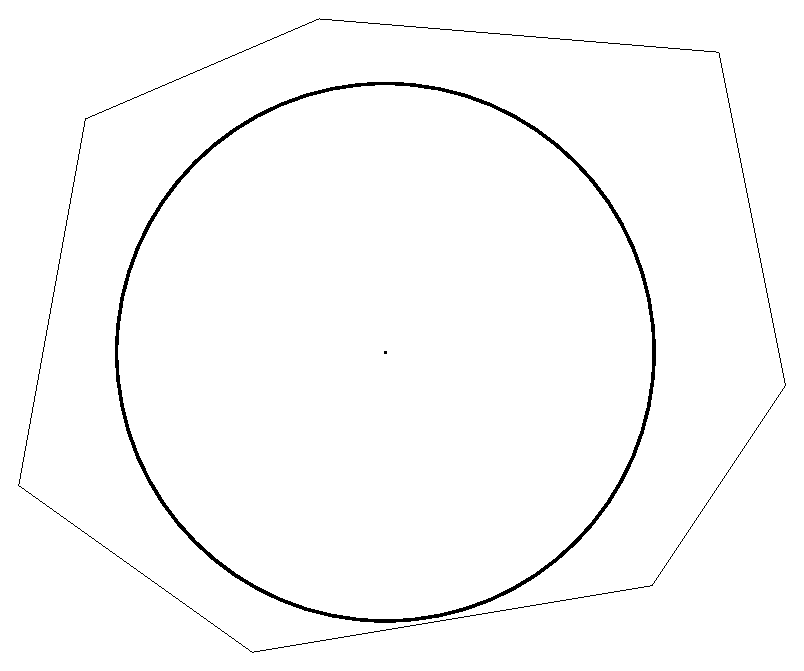
\includegraphics[scale=0.4]{2d/inter_voronoi_ball_2d_no_inter}
        \subcaption{No intersections}
        \label{fig:inter_voronoi_ball_2d:b}
    \end{minipage}
    \begin{minipage}{0.32\linewidth}
        \centering
        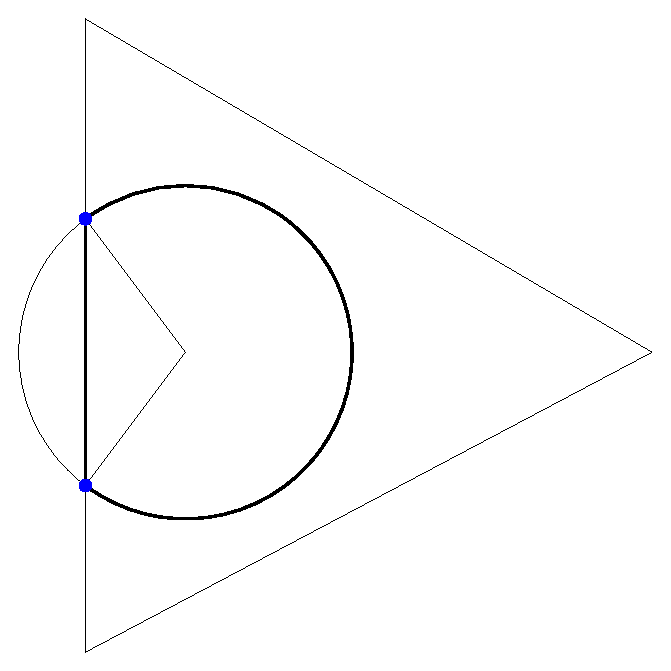
\includegraphics[scale=0.4]{2d/inter_voronoi_ball_2d_2_inter}
        \subcaption{2 intersections}
        \label{fig:inter_voronoi_ball_2d:c}
    \end{minipage}

   \caption{Different cases for the intersection between a Voronoi cell and a sphere}
   \label{fig:inter_voronoi_ball_2d}
\end{figure}

We use \texttt{CGAL} to compute the Delaunay triangulation of our point set: it
is the dual of the Voronoi diagram. A triangle in the Delaunay
triangulation corresponds to a vertex in the Voronoi diagram, an edge
corresponds to an edge, a vertex corresponds to a face...

Given this triangulation, we can compute the vertices composing the boundary of
the  Voronoi cell (in bold in the figures \ref{fig:inter_voronoi_ball_2d}) of a
point by doing the following:
\begin{enumerate}
    \item Access the neighbouring faces of a vertex using the
        \texttt{incident\_faces} method.
    \item Compute the Voronoi vertices (circumcenters) of these faces using the
        \texttt{dual} method.
\end{enumerate}

In 2D, consider the intersection of the Voronoi cell of $ p $ and a ball $ B(p,
r) $. The boundary of this intersection is composed of segments and circular
arcs. There are two types of points connecting those elements: some are Voronoi
vertices (in red) and some are intersections of Voronoi edges and circles (in
blue). We will refer to the red points as the interior points and to the blue
ones as intersection points.

First, we construct an array of all the points composing the boundary of the
intersection. In order to do this, we loop over the vertices composing the
Voronoi cell: for any Voronoi vertex $ v $, we have access to the next one in
the counterclockwise order and so we construct the corresponding edge. We check
whether this edge intersects the ball or not and we construct the intersection
point if necessary.. In parallel, we maintain a boolean indicating whether the
current point is interior or not. By doing that, we can construct an ordered
list of all the points present on the boundary of the intersection.

Then, we loop over this array, for any points $ u $ and $ v $, we can construct
the edge $ e = uv $. Depending on whether the points $ u $ and $ v $ are
interior or not, the contribution of $ e $ to the global area will be different:
\begin{itemize}
    \item if $ u $ and $ v $ are interior points, we add the area of triangle $ upv $.
    \item if $ u $ or $ v $ is interior point, we add the area of triangle $ upv $.
    \item if $ u $ and $ v $ are intersection points, then if they belong to the
        same Voronoi edge, we add the area of triangle $ upv $. If not, we add the
        area of angular sector $ \vec{pu}, \vec{pv} $.
\end{itemize}

Some special cases need to be handled:
\begin{itemize}
    \item the boundary of the Voronoi cell is entirely outside the ball (i.e.
        there are no intersection), then we add $ \pi r^2 $ to the area of the
        union (see \ref{fig:inter_voronoi_ball_2d:b}).
    \item the boundary consists of two intersection points $ p $ and $ q $, then
        we add the triangle $ pvq $ and the angular sector $ \vec{vp}, \vec{vq}
        $ (see \ref{fig:inter_voronoi_ball_2d:c}).
    \item there is only one point on the boundary (can happen if adjacent balls
        are tangential), then we add $ \pi r^2 $.
\end{itemize}

This algorithm allows us to compute exactly the area of a union of disks.

We use the same technique for computing the perimeter of the boundary of the
intersection except that if there are no intersection then the perimeter is $ 2
\pi r $ and instead of adding triangles areas or angular sectors, we only add
length of circular arcs.

% {{{3 IMPLEMENTATION DETAILS
\paragraph{Implementation details}

For the implementation, we used different libraries: \texttt{CGAL} which is a
C++ library that offers all the basic geometric types (point, vector, line,
plane..), data structures and algorithms (triangulations...). We also used
\texttt{Eigen} which is a C++ linear algebra library which provides types such
as vector, matrix and manipulation operations. We used \texttt{Qt} for the GUI
programming.

The main difficulty here was to compute the intersection between a Voronoi cell
and a circle. The Voronoi cell is computed using its dual graph: the Delaunay
triangulation. The intersection procedure was described previously.

We also used the automatic differentiation technique (see the appendix
\ref{appendix:ad}): it allowed us to only worry about the computation of the
area and not of its gradient.

% {{{1 EXPERIMENTS
\section{Experiments}

% {{{2 GRADIENT
\subsection{Gradient}

In this section, we will study the gradient of the area of union of balls, the
perimeter of the boundary. We used the automatic differentiation technique
described in the appendix \ref{appendix:ad} to compute the gradient of the
previously computed area.

See the figures \ref{fig:gradients_area_2d} for a few examples of such gradients
for different input point sets. The colour of the vector depend on the norm of
the gradient: the bigger the gradient is, the redder the vector will be.

\begin{figure}[h]
    \centering

    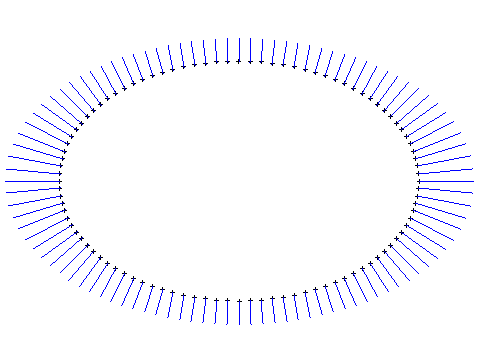
\includegraphics[scale=0.3]{2d/area/ellipse-100-01-15-gradients}
    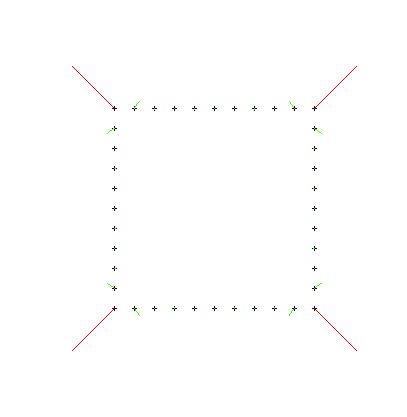
\includegraphics[scale=0.3]{2d/area/square-40-001-100-gradients}
    \subcaption{Gradients of the area for points sampled on an ellipse / a square}
    \label{fig:gradients_area_2d}
\end{figure}

We did the same thing using the gradient of the perimeter of the boundary on the
same point clouds (see the figures \ref{fig:gradients_perimeter_2d}).

\begin{figure}[h]
    \centering
    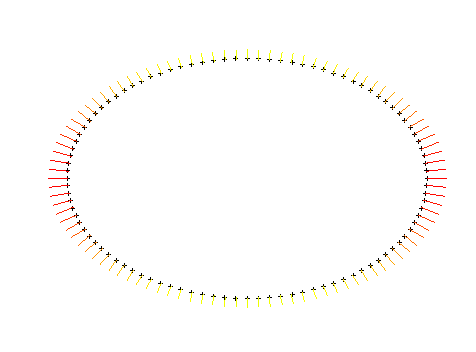
\includegraphics[scale=0.3]{2d/perimeter/ellipse-100-01-15-gradients}
    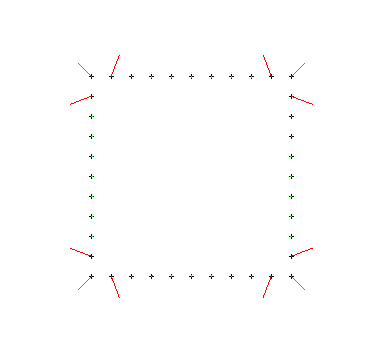
\includegraphics[scale=0.3]{2d/perimeter/square-40-001-100-gradients}

    \subcaption{Gradients of the perimeter for points sampled on an ellipse / a square}
    \label{fig:gradients_perimeter_2d}
\end{figure}

In the previous screenshots, we observe that the gradients are in the same
direction as the normals to the underlying curve. This is the case if the radius
of the balls are big enough and if the sampling is sufficiently uniform. Also,
the norm of these gradients is related to the mean curvature of the underlying
curve (see proposition \ref{prop:gradient-mean-curvature}).

% {{{2 MEAN CURVATURE ESTIMATION
\subsection{Mean curvature estimation}

In this section, we experimentally check in a particular case that we can
estimate the mean curvature on a point set using the norm of the gradients of
the area of a union of disks. The theoretical justification is given in chapter
\ref{chapter:theory}.

We run our tests on a sampled ellipse whose major and minor axes are $ a $ and $
b $. We can parametrize this ellipse by :
$$
\begin{cases}
    x(t) &= a \cos (t) \\
    y(t) &= b \sin (t)
\end{cases}
\text{ for t } \in [ 0, 2\pi ]
$$

We recall the formula for computing the curvature of a parametrized curve:
$$ \kappa(t) = \frac{x'(t) y''(t) - y'(t) x''(t)}{(x'^2(t) +
    y'^2(t))^{\frac{3}{2}} } $$

For an ellipse, we obtain:
$$ \kappa(t) = \frac{ab}{(a^2 \cos^2(t) + b^2 \sin^2(t))^{\frac{3}{2}} } $$

We compare this for $ t = \frac{2 k \pi}{N} $ for $ k = 0 \ldots N - 1 $ with
the computed ones where $ N $ is the number of samples.

The figure \ref{fig:2d-curvature-ellipse} represent the computed gradients mapped
to a colour ramp (from green to red). We observe that the gradients are more
important where the curvature is higher and are collinear to the outward normals
of the underlying curve.

\begin{figure}[h]
    \centering

    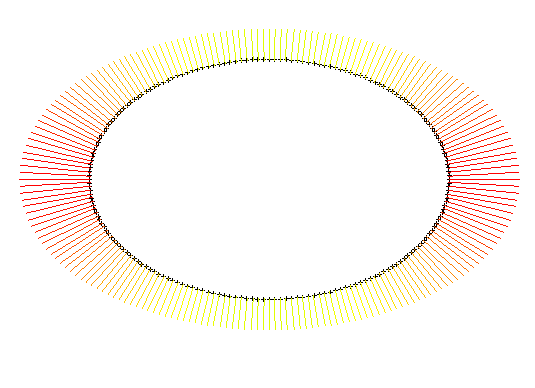
\includegraphics[scale=0.3]{2d/area/curvature-ellipse-200-15}
    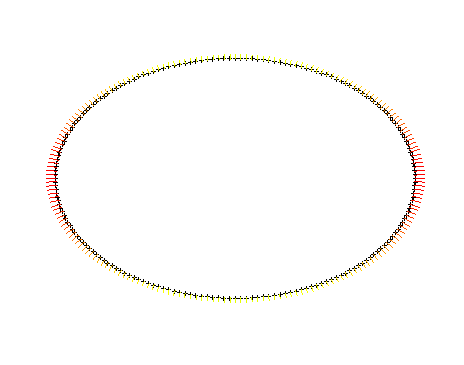
\includegraphics[scale=0.3]{2d/perimeter/curvature-ellipse-200-15}
    \caption{Computed curvatures on an ellipse using gradients of the area /
        perimeter}
    \label{fig:2d-curvature-ellipse}
\end{figure}

% TODO: pictures

Now, we study the absolute difference between the computed and expected
curvatures for different choices of gradients (area, perimeter of the boundary,
weighted...), see the figure \ref{fig:2d-curvature-error-ellipse}.

\begin{figure}[h]
    \centering

    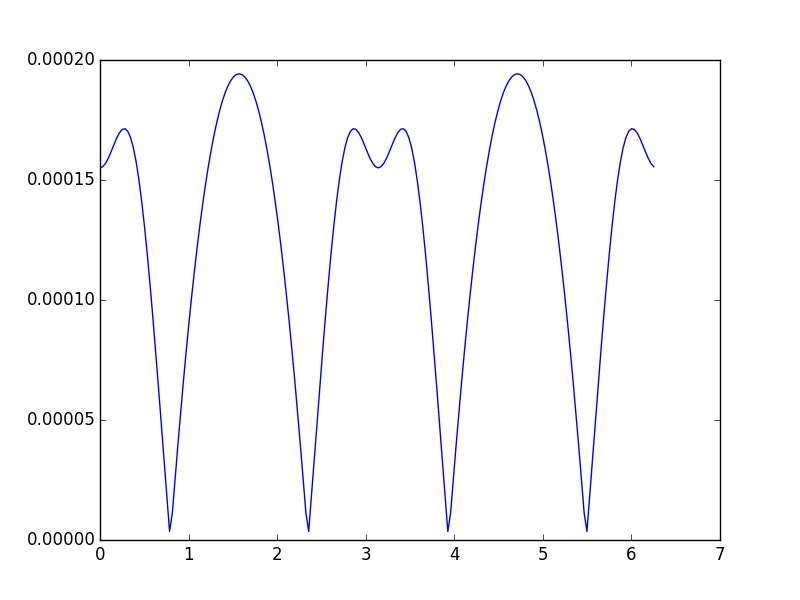
\includegraphics[scale=0.3]{2d/area/curvature-error-ellipse-200-05}
    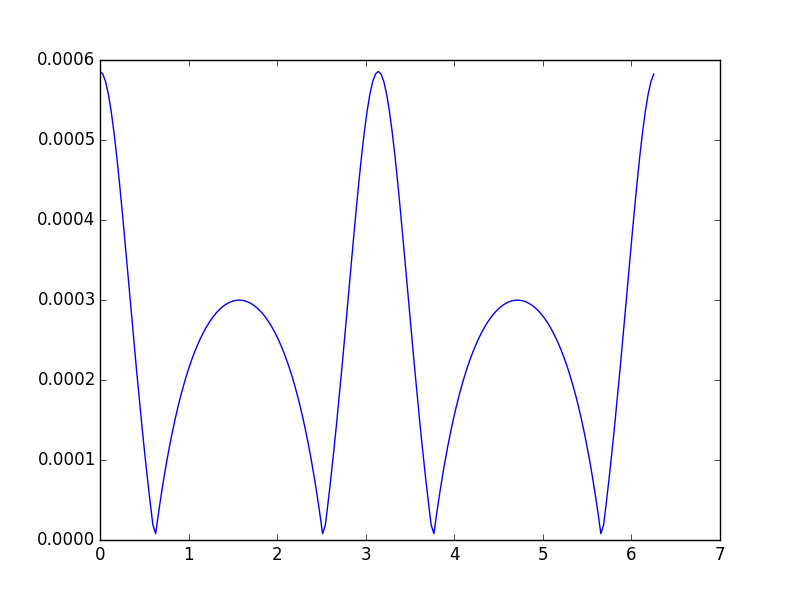
\includegraphics[scale=0.3]{2d/perimeter/curvature-error-ellipse-200-05}
    \caption{Error between the curvatures on an ellipse using gradients of the
        area / perimeter}
    \label{fig:2d-curvature-error-ellipse}
\end{figure}

We see that the error is less important for the area.

% {{{2 DISCRETE MEAN CURVATURE FLOW
\subsection{Discrete Mean Curvature Flow}

Now, we will be interested in approximating the continuous mean curvature flow
by applying a gradient descent algorithm in order to minimize a functional $ E
$.

This gradient descent will be done using a constant timestep (Euler explicit
scheme).

We will also be interested in weighted versions of functionals: we can weight
the gradient of the area by the perimeter of the visible part (the circular arcs
composing the intersection of the Voronoi cell and the ball) of the restricted
region. But by doing that, we can divide by $ 0 $ so we need to choose a small
time step in order to avoid the case where a point does not see anything.

% TODO

We did some experiments to validate our results: we first compared the two
gradient flows (area and perimeter of the boundary) to a set of points uniformly
sampled on an ellipse: figures \ref{fig:ellipse_area_flow} and
\ref{fig:ellipse_perimeter_flow}.

% TODO: ajouter convergence vers cercle
\begin{figure}[h]
    \centering

    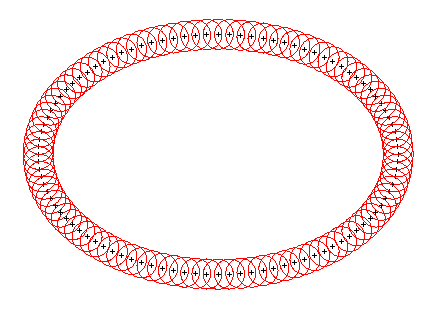
\includegraphics[scale=0.3]{2d/ellipse-balls-15}
    \subcaption{Minkowski sum of an ellipse and balls of radius $ 15 $}

    \includegraphics[scale=0.3]{2d/area/ellipse-100-01-15}
    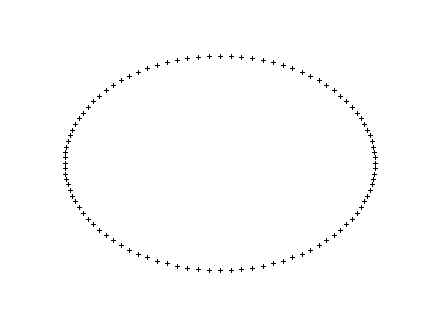
\includegraphics[scale=0.3]{2d/area/ellipse-100-01-15-100}
    \subcaption{Area flow of an ellipse: 0 / 100 iterations with a timestep of $ 0.1 $}
    \label{fig:ellipse_area_flow}

    \includegraphics[scale=0.3]{2d/perimeter/ellipse-100-01-15}
    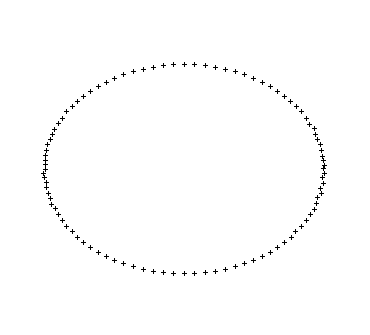
\includegraphics[scale=0.3]{2d/perimeter/ellipse-100-01-15-100}
    \subcaption{Perimeter flow of an ellipse: 0 / 100 iterations with a timestep of $ 0.5 $}
    \label{fig:ellipse_perimeter_flow}

    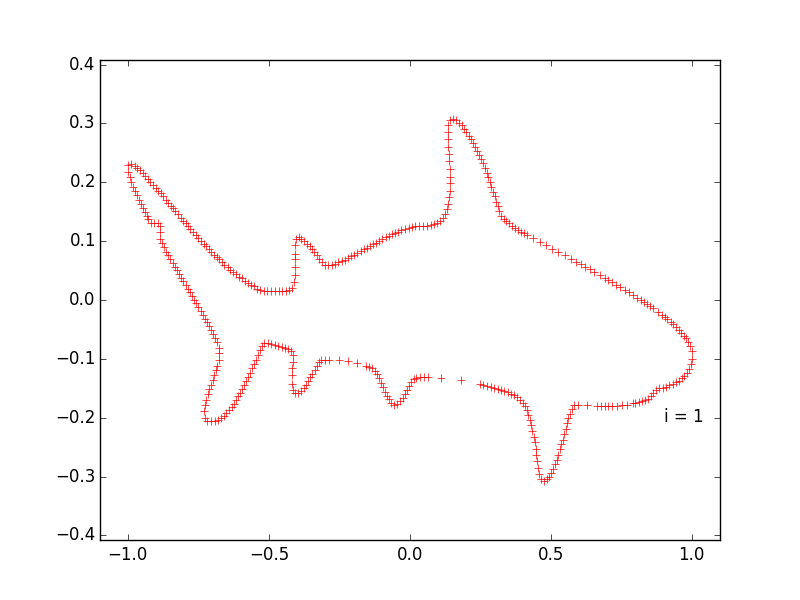
\includegraphics[scale=0.22]{2d/perimeter/shark-0}
    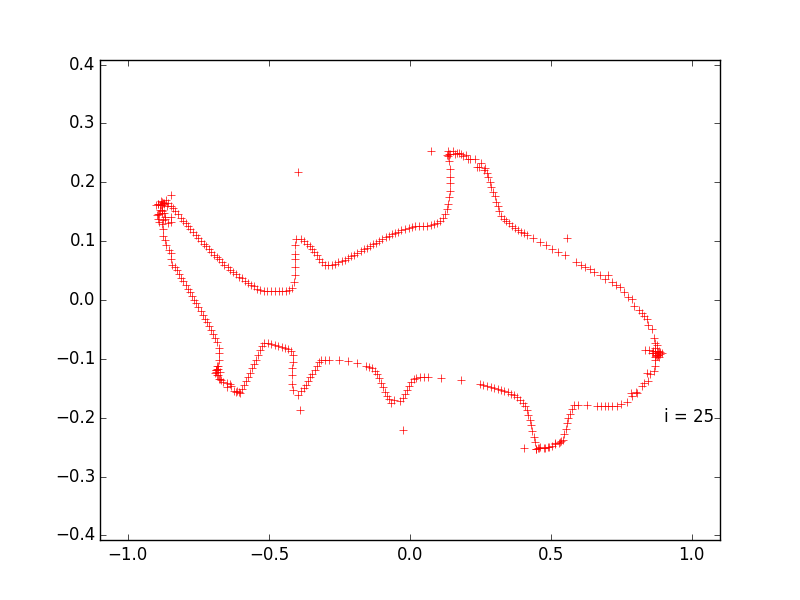
\includegraphics[scale=0.22]{2d/perimeter/shark-24}
    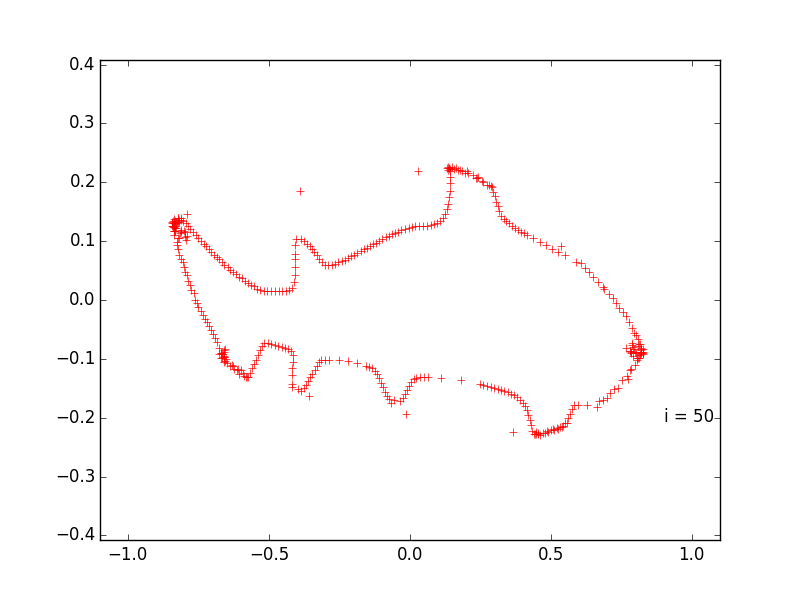
\includegraphics[scale=0.22]{2d/perimeter/shark-49}
    \subcaption{Perimeter flow of a shark: 0 / 25 / 50 iterations with a
        timestep of $ 0.05 $}

    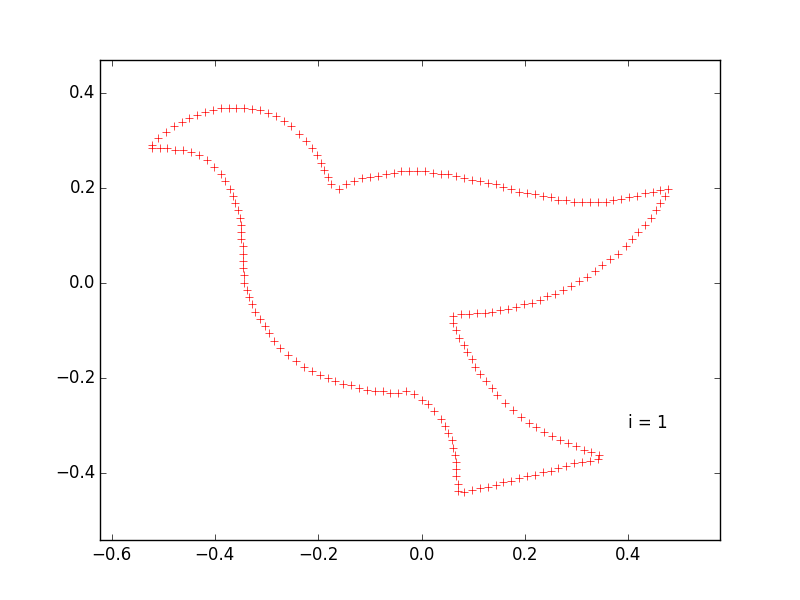
\includegraphics[scale=0.22]{2d/perimeter/bird-0}
    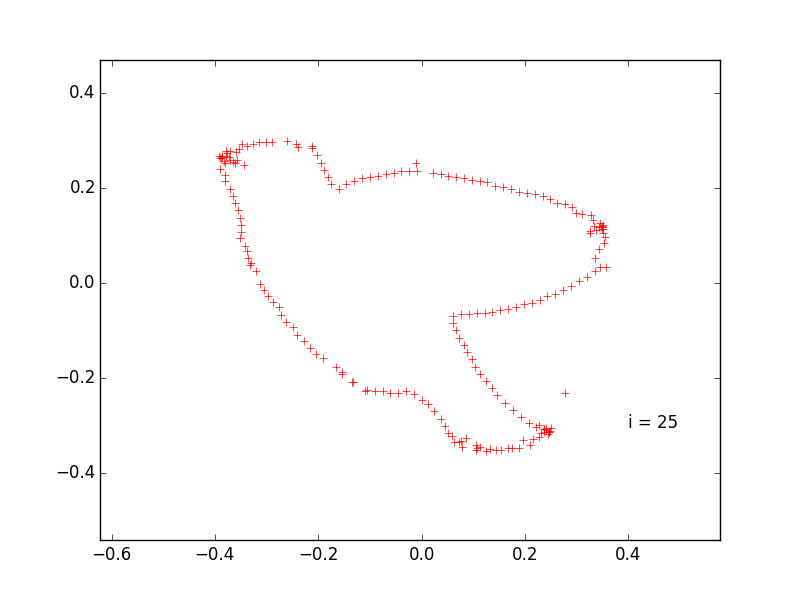
\includegraphics[scale=0.22]{2d/perimeter/bird-24}
    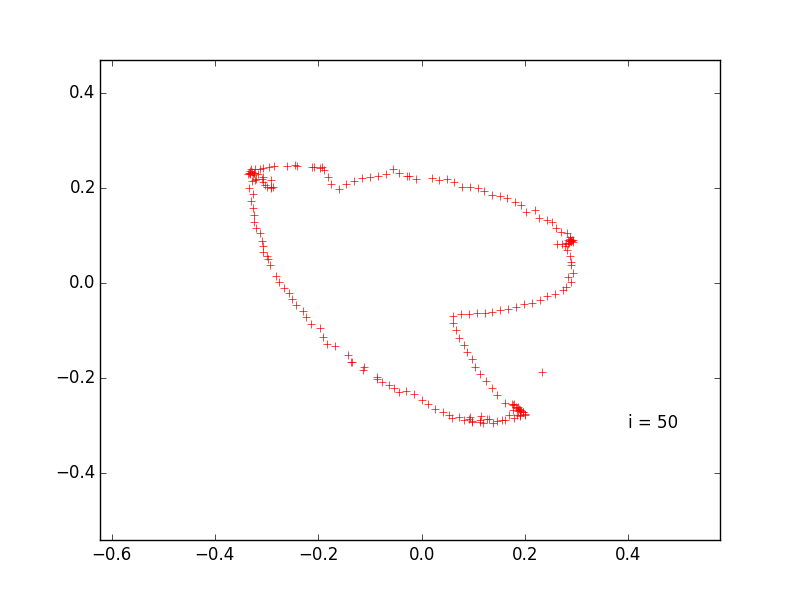
\includegraphics[scale=0.22]{2d/perimeter/bird-49}
    \subcaption{Perimeter flow of a bird: 0 / 25 / 50 iterations with a
        timestep of $ 0.05 $}
    \label{fig:shark_perimeter_flow}
\end{figure}

We test the smoothing property of our flow on points sampled on a square, see
the figure \ref{fig:area_perimeter_flow_square}. We can clearly see that our
discrete flow smooth the corners of the square.

\begin{figure}[h]
    \centering
    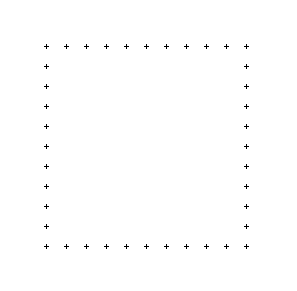
\includegraphics[scale=0.3]{2d/square-0}
    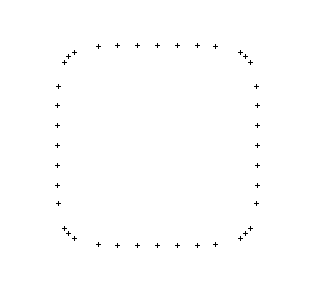
\includegraphics[scale=0.3]{2d/area/square-area-4-15-01}
    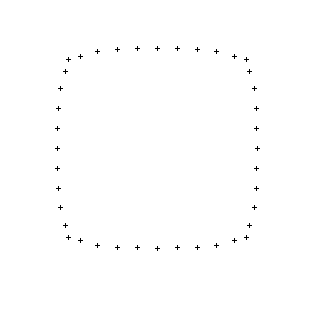
\includegraphics[scale=0.3]{2d/perimeter/square-perimeter-10-15-05}
    \caption{Area / perimeter flow on a square}
    \label{fig:area_perimeter_flow_square}
\end{figure}

We also verify that the area of the union of balls decreases with the number of
iterations, see the figure \ref{fig:area_time_decrease}.

\begin{figure}[h]
    \centering
    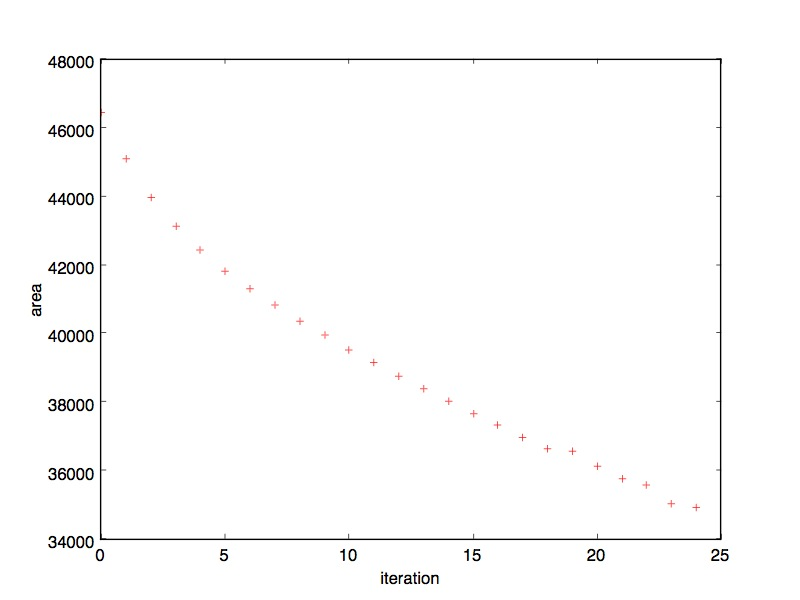
\includegraphics[scale=0.3]{2d/values-square-area}
    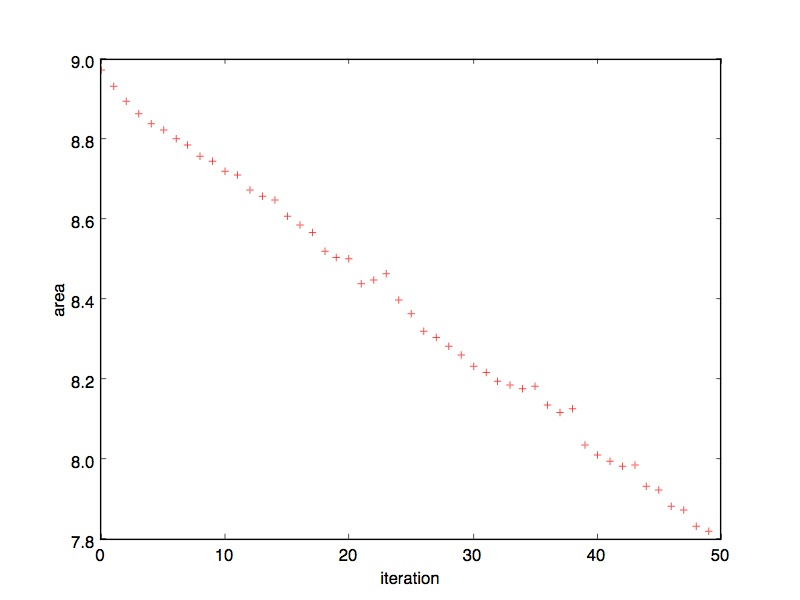
\includegraphics[scale=0.3]{2d/values-ellipse-perimeter}
    \caption{Evolution of the area on different point clouds with the area
        flow : square / ellipse}
    \label{fig:area_time_decrease}
\end{figure}

Next, we add some outliers around the ellipse and observe the effects of the two
flows: see the figures \ref{fig:ellipse_outliers_area_flow} and
\ref{fig:ellipse_outliers_perimeter_flow}. We see that the outliers are
"swallowed" by the initial point set in both cases. But, for the area flow, a
hole is created at the same place where the outliers were added.

\begin{figure}[h]
    \centering

    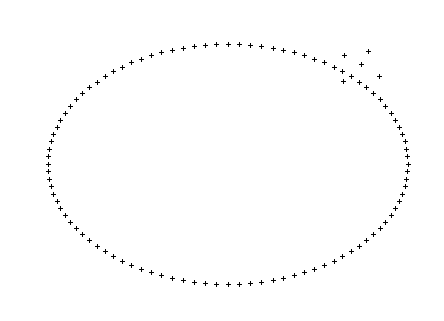
\includegraphics[scale=0.3]{2d/area/ellipse-100-01-15-outliers}
    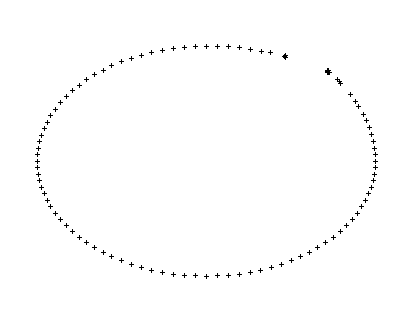
\includegraphics[scale=0.3]{2d/area/ellipse-100-01-15-outliers-40}
    \subcaption{Area flow of an ellipse with outliers: 0 / 40 iterations with a
        timestep of $ 0.1 $}
    \label{fig:ellipse_outliers_area_flow}

    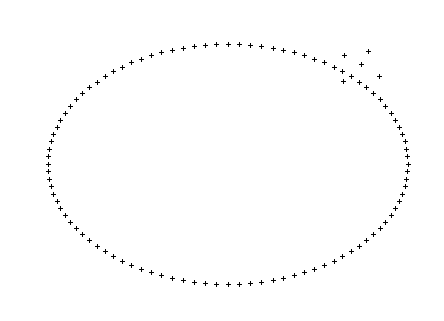
\includegraphics[scale=0.3]{2d/perimeter/ellipse-100-1-15-outliers}
    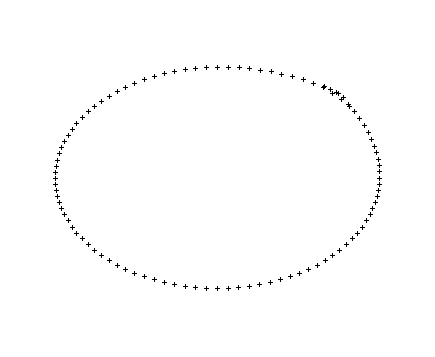
\includegraphics[scale=0.3]{2d/perimeter/ellipse-100-1-15-outliers-100}
    \subcaption{Perimeter flow of an ellipse with outliers: 0 / 100 iterations
        with a timestep of $ 1 $}
    \label{fig:ellipse_outliers_perimeter_flow}
\end{figure}

Then, we added some Gaussian noise on these points to test the robustness of our
algorithm, see the figures \ref{fig:ellipse_noise_area_flow} and
\ref{fig:ellipse_noise_perimeter_flow}.

\begin{figure}[h]
    \centering

    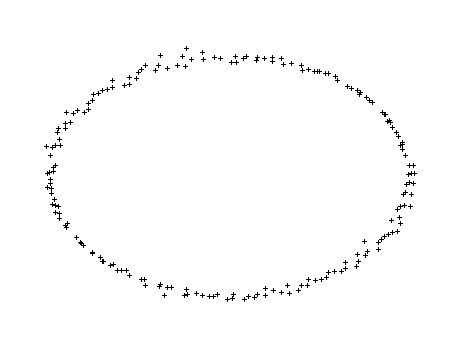
\includegraphics[scale=0.3]{2d/ellipse-noise-5-0}
    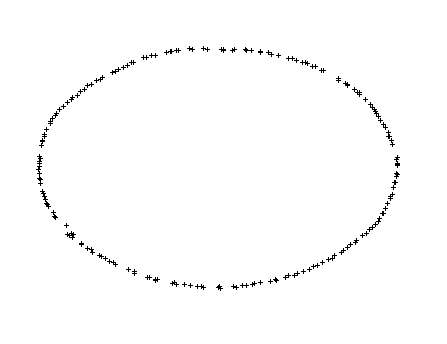
\includegraphics[scale=0.3]{2d/area/ellipse-noise-5-75}
    \subcaption{Area flow on a noised ellipse: 0 / 75 iterations with a timestep of $ 0.05 $}
    \label{fig:ellipse_noise_area_flow}

    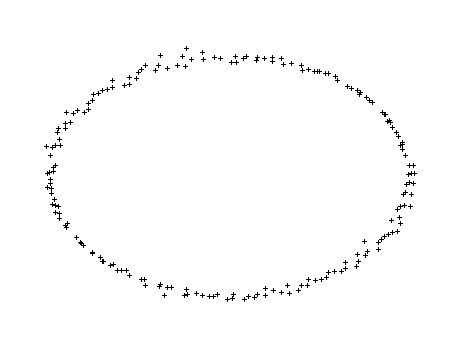
\includegraphics[scale=0.3]{2d/ellipse-noise-5-0}
    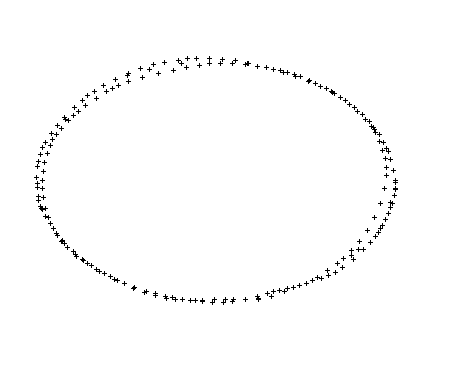
\includegraphics[scale=0.3]{2d/perimeter/ellipse-noise-5-75}
    \subcaption{Perimeter flow on a noised ellipse: 0 / 75 iterations with a timestep of $ 0.5 $}
    \label{fig:ellipse_noise_perimeter_flow}
\end{figure}

We notice that the gradient flow of the area may create holes in the point set
which is not the case for the gradient flow of the perimeter.

On the contrary, the gradient flow of the perimeter of the boundary will smooth
the point set while redistributing the points in an uniform way.

% TODO: explain why
This can be explained by looking on a simple case with two intersecting balls:
\begin{itemize}
    \item \textit{for the perimeter}: the gradients are directed towards the outside
        and so the balls will be merged because we can say, using the triangle
        inequality, that in order to minimize the perimeter the balls must come
        closer.
    \item \textit{for the area}: using the same reasoning, in order to minimize the area,
        it is possible that the gradients are oriented in opposite directions
        because the area gain may be more costly than moving the balls closer.
\end{itemize}

The chosen radius will also influence the smoothing: points which are too far
away from other points (at distance greater than the radius) will not move. The
bigger radius is, the more points will move in big groups. Indeed, the
radius indicates how to take the neighbours of a point into account. The more
neighbours we take into account, the more "global" the movement will be.

We also add varying oscillations to our ellipse in order to see the
adaptive part of the algorithm. We generate oscillations with one or two
amplitudes.

For one constant amplitude, see the figures \ref{fig:ellipse_osc_perimeter_flow} and
\ref{fig:ellipse_osc_area_flow} and for two different amplitudes see
\ref{fig:ellipse_osc2_area_flow} and \ref{fig:ellipse_osc2_perimeter_flow}.

\begin{figure}[h]
    \centering

    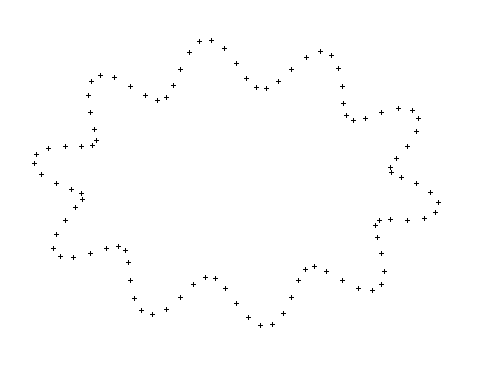
\includegraphics[scale=0.3]{2d/ellipse-osc-25-15-0}
    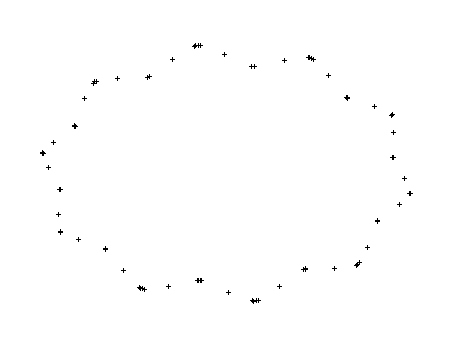
\includegraphics[scale=0.3]{2d/area/ellipse-osc-25-15-25}
    \subcaption{Area flow on an ellipse with oscillations (one amplitude) : 0 /
        25 iterations with a timestep of $ 0.05 $ and a radius of $ 15 $}
    \label{fig:ellipse_osc_area_flow}

    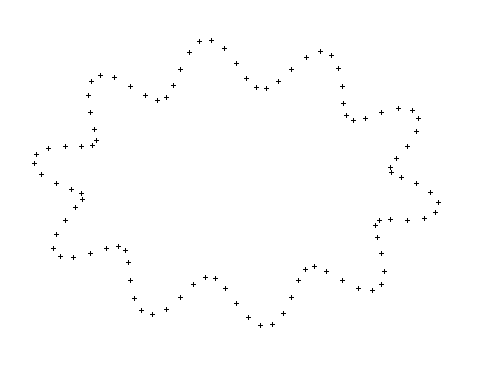
\includegraphics[scale=0.3]{2d/ellipse-osc-25-15-0}
    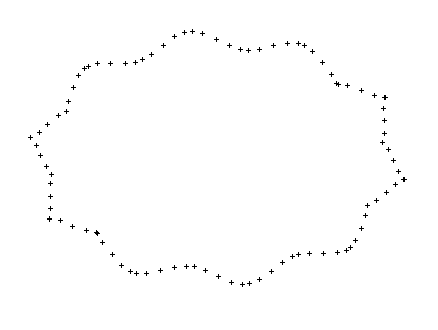
\includegraphics[scale=0.3]{2d/perimeter/ellipse-osc-25-15-50}
    \subcaption{Perimeter flow on an ellipse with oscillations (one amplitude):
        0 / 55 iterations with a timestep of $ 0.5 $ and a radius of $ 15 $}
    \label{fig:ellipse_osc_perimeter_flow}
\end{figure}

\begin{figure}[h]
    \centering

    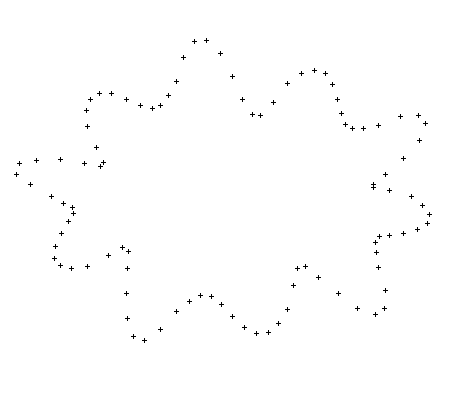
\includegraphics[scale=0.3]{2d/ellipse-osc2-20}
    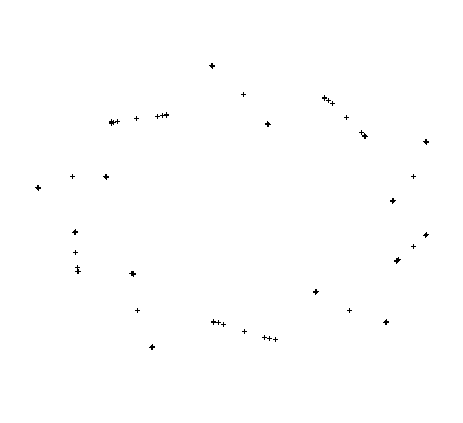
\includegraphics[scale=0.3]{2d/area/ellipse-osc2-20-15-25}
    \subcaption{Area flow on an ellipse with oscillations (two amplitudes): 0 /
        25 iterations with a timestep of $ 0.05 $ and a radius of $ 15 $}
    \label{fig:ellipse_osc2_area_flow}

    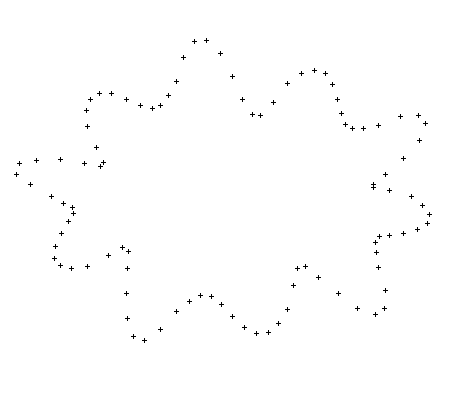
\includegraphics[scale=0.3]{2d/ellipse-osc2-20}
    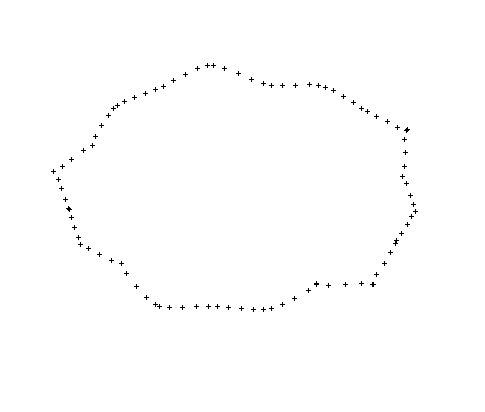
\includegraphics[scale=0.3]{2d/perimeter/ellipse-osc2-20-15-55}
    \subcaption{Perimeter flow on an ellipse with oscillations (two amplitudes)
        : 0 / 55 iterations with a timestep of $ 0.5 $ and a radius of $ 15 $}
    \label{fig:ellipse_osc2_perimeter_flow}
\end{figure}

% TODO: explain why

In another experiment we took points on a line segment and fixed the two points
of the extremities. Then, we applied our flow on this point set. We expect the
flow to smooth the point set: points should get closer and closer to an
uniformly sampled set of points. See the figures \ref{fig:line_fixed_area} and
\ref{fig:line_fixed_perimeter} for the results.

\begin{figure}[h]
    \centering

    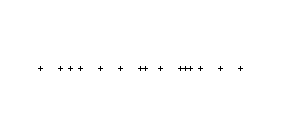
\includegraphics[scale=0.5]{2d/area/line-01-15-0}
    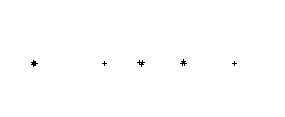
\includegraphics[scale=0.5]{2d/area/line-01-15-50}
    \subcaption{Area flow of points on a segment: 0 / 50 iterations with a timestep of $ 0.1 $}
    \label{fig:line_fixed_area}

    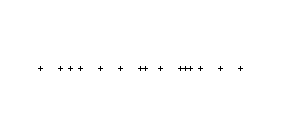
\includegraphics[scale=0.5]{2d/perimeter/line-05-15-0}
    \includegraphics[scale=0.5]{2d/perimeter/line-05-15-50}
    \subcaption{Perimeter flow of points on a segment: 0 / 50 iterations with a timestep of $ 0.5 $}
    \label{fig:line_fixed_perimeter}
\end{figure}

% TODO: explain why

% {{{1 CONCLUSION
\section{Conclusion}

In summary, the two flows (area and perimeter of the boundary) have the
following common properties:
\begin{itemize}
    \item Smooth the point set: remove the outliers / noise
    \item Can be used to estimate the mean curvature
\end{itemize}

But, there are differences between the two flows. The main one is that the area
flow has the tendency to create holes in the point cloud. This difference is
removed when we use the weighted versions of the flows.

% {{{1 ASSESSMENT
% \section{Assessment}

% In this chapter, we saw how to simulate discrete mean curvature flows by using
% the gradient of the volume of the $r$-offset of a point cloud.

% The methods used in this chapter are hard to extend in 3D but have already been
% done: see \cite{cazals2011computing}.

% Also, we want to use polyhedral (anisotropic) norms, a thing that the previous
% method does not allow since it only deals with intersection of a Voronoi cell
% and a ball and we need a way to intersect a Voronoi cell and a polygon.

% TODO:
% - description
% - résultats
% - bilan + transition

% vim: set spelllang=en :

\chapter{3D case}
\label{chapter:3d}

% {{{1 INTRODUCTION
\section{Introduction}

In this part, we focus on point clouds in 3D that sample a surface. Our goal is
to do the same work as the one done in 2D that is to say smooth the point cloud
using a mean curvature flow approach. This means computing the volume of a union
of balls centered at the points and move the points in the opposite direction to
the one given by the gradient of the volume. An algorithm for computing the
volume can be found in \cite{cazals2011computing}. Since we expect the same
results as in the 2D case (see Chapter \ref{chapter:theory} for a
justification), we preferred to focus to an other kind of flow: an anisotropic
one.

The idea of this flow is to replace the union of balls with a union of convex
polyhedra. The choice of the polyhedron will directly influence the directions
in which the points will be moved.

For doing that, we will replace the Euclidean ball $ B(0, 1) $ with a convex
polyhedron $ B_N(0, 1) $ which can be considered as the unit ball for a certain
norm $ N $. This norm will be called polyhedral (see Section
\ref{sec:polyhedral-norm}). The formula \ref{eqn:area-union-balls} remains valid
if we replace $ B(p, r) $ with $ B_N(p, r) $ and $ V $ by $ V_N $ (the Voronoi
diagram computed for the norm $ N $) but only if the points are in general
position. In Appendix \appendixref{appendix:voronoi-polyhedral-norm}, we study
some properties of the Voronoi diagram for a polyhedral norm. Indeed, see Figure
\ref{fig:3d-voronoi-cube} for a look at a particular case where the chosen
polyhedron is a cube (norm $ L^\infty $). We see that if we choose two aligned
points, the bisector is not a line anymore and so the Voronoi diagram does not
partition the plane anymore. Furthermore, the computation of the Voronoi cells
for a polyhedral norm is a tough work (see \cite{ma2000bisectors} for a thorough
study).

\begin{figure}[h]
    \centering

    \includegraphics[scale=0.5]{3d/voronoi-cube-non-aligned}
    \hspace{2cm}
    \includegraphics[scale=0.5]{3d/voronoi-cube-aligned}
    \caption{Bisector for the $ L^\infty $ norm: two non aligned points / two
        aligned points}
    \label{fig:3d-voronoi-cube}
\end{figure}

For computing the volume of $ \bigcup_{p \in P} B_N(p, r) $, we implemented two
different methods: a naive one and one based on inclusion-exclusion formula.  In
the naive one, we make the following approximation: instead of summing up over
all intersections $ V_N(p, P) \cap B_N(p, r) $, we sum up over all $ V(p, P)
\cap B_N(p, r) $. The influence of this choice under the functional we minimized
is described in Section \ref{sec:theory-3d-case}. We will see that the second
approached based on inclusion-exclusion formulae is also an approximated one.
There is also one method which is exact but we did not have the time to
implement it in our internship, it is based on 3D arrangements and overlays.

Firstly, we will define formally what we call a polyhedral norm. Then, we will
explain our naive method. Secondly, we will explain the inclusion-exclusion
formula we used in our second method. Then, we will talk about the choices we
made for the implementation and finally, we will run experiments to validate our
expectations.

% {{{1 POLYHEDRAL NORM
\section{Polyhedral norm}
\label{sec:polyhedral-norm}
A polyhedral norm is a function $ N $ defined as follows:

\begin{equation}
    \forall x \in \mathbb{R}^d,~ N(x) = \max_{i} (x | v_i)
\end{equation}
where the $ v_i $ are given vectors from $ \mathbb{R}^d $. This definition
implies that the unit ball for the norm $ N $ is a polyhedron. Indeed, if $ x
\in B_N(0, 1) $, then :

$$ N(x) \leq 1 \Longleftrightarrow \forall i,~(x | v_i) \leq 1 $$

So, the unit ball is defined by linear constraints. More precisely, it is an intersection
of half-spaces and so is a convex polyhedron $ K $. The vectors $ v_i $ are the
normal vectors to the facets of $ K $. We will denote by $ B_K(0, 1) $ the unit
ball defined by the convex polyhedron $ K $.

% {{{1 VOLUME OF A UNION OF POLYHEDRA
\section{Volume of a union of polyhedra}

In this section, we will show how to compute an approximation of the volume of
a union of polyhedra using two different methods: a naive one and one based on
inclusion-exclusion formula.

% {{{2 NAIVE METHOD
\subsection{Naive method}
We want to compute :

\begin{equation}
    Vol(\bigcup_{p \in P} B_N(p, r)) = \sum_p Vol(\bigcup_p B_N(p, r) \cap V(p, P))
\end{equation}

The idea of this method is to approximate $ Vol(\bigcup_p B_N(p, r) \cap V(p,
P)) $ by $ Vol(B_N(p, r) \cap V(p, P)) $. Then, we just have to compute the
intersection of half-spaces (see Section \ref{sec:3d-implementation} for
details). It is an approximation because, for example, if we want to compute the
perimeter of the boundary of squares in 2D, there is a difference between what
we want to compute and what we actually compute (see Figure
\ref{fig:3d-inclusion-exclusion-squares}): our computation is just an
approximation.

\begin{figure}[h]
    \centering

    \includegraphics[scale=0.8]{3d/3d_perimeter_squares_truth}
    \hspace{2cm}
    \includegraphics[scale=0.8]{3d/3d_perimeter_squares}
    \caption{In green, what we want and in red what we actually compute}
    \label{fig:3d-inclusion-exclusion-squares}
\end{figure}

% {{{2 INCLUSION-EXCLUSION FORMULA
\subsection{Inclusion-exclusion formula}

The inclusion-exclusion formula is a well-known formula which can be used to
compute the indicator function of a union of sets: given a finite number of sets
$ A = \{ A_1, \ldots, A_N \} $, we have:

\begin{equation}
    \indicator{\bigcup A_i} = \sum_{\emptyset \neq X \subseteq A} (-1)^{card X -
        1} \indicator{\bigcap X}
\end{equation}

This formula can also be expressed using the notion of nerve as shown in
\cite{attali2007inclusion}. We define the nerve of $ A = \{ A_x, x \in X \} $ to
be the simplicial complex \footnote{A simplicial complex is a generalization of
    a triangulation: it is a collection of simplices like vertices, edges,
    triangles, tetrahedra...} where a simplex $ \sigma $ exists between $ x_1
\ldots, x_k $ if $ \bigcap\limits_{i=1}^k A_{x_i} \neq \emptyset $. Then, we can
write the inclusion-exclusion formula as:

$$ \indicator{\bigcup A_x} = \sum_{\sigma \in Nerve(A)} (-1)^{\dim \sigma}
\indicator{\bigcap \sigma} $$
$ \sigma $ represents any simplex in the nerve. Its dimension is defined as: $
\dim \sigma = card \sigma - 1 $. If we consider a union of polyhedra, we can write a similar formula:

\begin{equation}
    \indicator{\bigcup B_N(p, r)} = \sum_{\sigma \in Nerve(\mathcal{B}_N)} (-1)^{\dim \sigma}
    \indicator{\bigcap \sigma}
    \label{eqn:incl_excl_simplices}
\end{equation}
where $ \mathcal{B}_N $ is the collection of all balls $ B_N(p, r), p \in P $.

Now, since the nerve can be a really big object, we want to restrict the
computation to what we call the $\alpha$-complex of a set of points:

\begin{definition} The $\alpha$-complex of a set of points $ X $ denoted by $
    Del(X, \alpha) $ is a subset of the Delaunay triangulation. To each simplex
    of the Delaunay triangulation, we can associate a characteristic
    radius: the radius of the smallest empty circle containing the simplex.

    Now, the $\alpha$-complex contains all the simplices of the Delaunay
    triangulation whose characteristic radius is smaller than $\alpha$.
\end{definition}

Now, we can ask if the formula \ref{eqn:incl_excl_simplices} is still valid if
we replace $ Nerve(\mathcal{B}_N) $ by $ Del(P, r) $.

If we want to prove this assertion, we may use the technique used to prove the
inclusion-exclusion formula for a union of balls. The proof starts by defining
the subcomplex $ L_p $ induced by a vertex $ p $.  We consider all the
polyhedrons that contains a given point $ x $ and we construct the nerve of it.
Formally, $ L_x = Nerve(\{ B_N(p, r),~x \in B_N(p, r)\}) $.

Then, when we evaluate the indicator function at $ x $ of the union, we can
decompose it in two parts: simplices of $ L_x $ and the other ones.

\begin{align*}
    \indicator{\bigcup B_N(p, r)}(x) &= \sum_{\sigma \in L_x} (-1)^{\dim \sigma}
    \indicator{\bigcap \sigma}(x) + \sum_{\sigma \notin L_x} (-1)^{\dim \sigma}
    \underbrace{\indicator{\bigcap \sigma}(x)}_{= 0 \text{ since } x \notin
        \sigma} \\
    &= \sum_{\sigma \in L_x} (-1)^{\dim \sigma} \\
    &= \chi(L_x)
\end{align*}

Here, $ \chi $ is the Euler characteristic.

Now, if we show that $ L_x $ is contractible (can be continuously deformed to a
point), we know that $ \chi(L_x) = 1 $. Obviously, we also have $
\indicator{\bigcup B_N(p, r)}(x) = 0 $ if $ x $ is not in the union and we will
conclude that the formula \ref{eqn:incl_excl_simplices} is true. But it appears
that there exists cases where the formula is not correct: see Figure
\ref{fig:incl_excl-examples}. In this figure, we can see that in the
$\alpha$-complex for the $ L^\infty $ norm, the triangle does not exist. It
means that in the formula the intersection between the three squares will not be
taken into account and so the final result will be incorrect. During this
internship, we did not have the time to estimate the error made by using this
formula.

\begin{figure}[h]
    \centering
    \includegraphics[scale=0.7]{3d/inclusion-exclusion-counter-l2}
    \hspace{2cm}
    \includegraphics[scale=0.7]{3d/inclusion-exclusion-counter-linfty}
    \caption{Counter example where the formula is not correct, in red the
        $ L^2$ $\alpha$-complex and in green the $ L^\infty$ $\alpha$-complex.}
    \label{fig:incl_excl-examples}
\end{figure}

% {{{1 IMPLEMENTATION DETAILS
\section{Implementation details}
\label{sec:3d-implementation}

In this section, we will describe briefly how we implemented the two methods
previously described.

The libraries used are the same as the ones used in the 2D case except for the
rendering part: in 2D, we used a custom \texttt{QWidget} and in 3D, we choose to
use \texttt{QGLViewer}, an \texttt{OpenGL} based renderer.

\paragraph{Intersection computation}

For both methods, we need a way to compute intersection of half-spaces: for
the first one, we need to compute the intersection of a Voronoi cell and a
convex polyhedron and for the second one, we need to compute intersections of
convex polyhedra.

For the first method, the naive one, a Voronoi cell is represented implicitly as
a list of half-spaces (the planes defining the boundary of the cell).
Half-spaces are computed using the Delaunay triangulation. If we want to compute
the Voronoi cell of $ p $, we look at the neighbours in the Delaunay
triangulation of $ p $. Then, for every neighbour $ v $, the corresponding
half-space is the positive part of the bisector plane between $ p $ and $ v $.
The latter is the  plane passing through the midpoint of the segment $ [p, v] $
and whose normal vector is $ \vec{pv} $. Since the order of the traversal of the
vertices of the Delaunay triangulation is not, in general, the same as the
insertion one, we need to associate an index to a point (using a simple
\texttt{std::map}).

Then, a convex polyhedron $ K $ represents the unit ball for the polyhedral norm
$ N $ defined by $ K $. It is internally represented as a list of normal vectors
of each of its facets. Using this representation, one can compute the translated
polyhedron $ B_N(p, r) $ for a point $ p $ and a radius $ r $ by noticing that
it is the intersection of the half-spaces: $ \forall n,~ n_x x + n_y y + n_z z -
(p | n) - r \leq 0 $ where $ n $ is a normal vector of a facet.

In order to construct this intersection, we used the duality which allows us to
replace the computation of the intersection by the computation of the convex
hull (see \cite{preparata1979finding}) of the dual points: at each half-space, we
can associate a dual point and conversely.

Programmatically, we compute this intersection in the following manner:
\begin{enumerate}
    \item Compute the dual points while remembering which point is associated to
        which plane.
    \item Compute the convex hull of these dual points, it gives us a dual
        polyhedron. To each vertex, we associate the corresponding primal plane.
    \item To compute the primal polyhedron:
        \begin{enumerate}
            \item We first compute the primal vertices which are the dual of the
                dual facets: each dual facet has at least 3 vertices. We know
                the corresponding primal planes for these vertices.  Then, the
                corresponding primal vertex is the intersection of these 3
                planes.
            \item Secondly, the primal facets are constructed by circulating
                around the dual vertices. Each time there is an edge between two
                dual vertices, there is an edge between the two corresponding
                primal ones.
        \end{enumerate}
\end{enumerate}

See Appendix \appendixref{appendix:code-intersection} for a simplified version
of this algorithm:

For the second method, we also need a way to compute the $\alpha$-complex of a
set of points. This can be done using the \texttt{Alpha\_shapes\_3} package of
\texttt{CGAL} and the associated classification methods.

\paragraph{Automatic Differentiation integration}

Let's now explain in more details the integration of the automatic
differentiation tool. \texttt{CGAL} has the particularity to make easy for the
programmer to change the number type by using the concept of a \emph{Kernel}. A
\emph{Kernel} is a class that describes how numbers are stored in memory, how we
can construct things (like points, planes, bisectors...) and how to evaluate
predicates on objects (collinearity test, coplanarity test...).

There are multiple predefined kernels but we will quickly talk about two
particular ones. \texttt{Simple\_cartesian<NT>} is the most basic one: a number
will just be represented by \texttt{NT} and so it has inexact predicates
evaluation and inexact constructions.

\texttt{Exact\_predicates\_inexact\_constructions\_kernel} (in short
\texttt{Epick}) is a Kernel which use a technique called \emph{filtering} to
ensure the predicates are always evaluated in an exact manner. In short, the
predicate is first evaluated in an inexact way using interval arithmetic.  Then,
if the predicate, for example, has to check whether a value is zero or not then,
using interval arithmetic, it will need to check whether the resulting interval
contains zero or not. If this interval does not contains zero, then a decision
can be made. Otherwise, the computation is redone but this time using exact
arithmetic which, in all cases, will return an answer.

For the automatic differentiation, we replaced the \texttt{NT} type with our
custom class \texttt{AD}. \texttt{AD} is a class with two members: a value and a
vector of derivatives. It overloads all the classical arithmetic operations and
some mathematical functions (\texttt{sqrt}, \texttt{atan2}...). For example, the
implementation of \texttt{sqrt} for AD looks like this:
\lstinputlisting[language=C++]{code/sqrt_AD.h}

Then, for interfacing \texttt{AD} with \texttt{CGAL}, we choose the
\texttt{Simple\_cartesian<AD>} kernel. The choice of \texttt{Simple\_cartesian}
may seem inappropriate because the constructions are inexact but it is enough
for our applications.

% TODO

% {{{1 EXPERIMENTS
\section{Experiments}

% TODO

We compare the two different methods using various polyhedrons as base and
various point clouds.

We can choose for the polyhedron a sufficiently discretized sphere. We expect
the result to be the same as in the 2D case: gradients oriented like the outward
normal with a norm proportional to the mean curvature.

The figures \ref{fig:3d-mean-curvature-sphere-cube} give an example where the
point cloud is a sphere and the polyhedron is a cube.

\begin{figure}[h]
    \centering
    \begin{minipage}{0.32\linewidth}
        \centering
        \includegraphics[scale=0.35]{3d/sphere-polyhedron-200}
        \subcaption{Discretized sphere with 200 planes}
    \end{minipage}
    \begin{minipage}{0.32\linewidth}
        \centering
        \includegraphics[scale=0.3]{3d/sphere-1000}
        \subcaption{Initial point cloud: 1000 points on a sphere}
    \end{minipage}
    \begin{minipage}{0.32\linewidth}
        \centering
        \includegraphics[scale=0.3]{3d/sphere-sphere-1000-05}
        \subcaption{Gradients of the volume}
    \end{minipage}
    \caption{Sphere / cube}
    \label{fig:3d-mean-curvature-sphere-cube}
\end{figure}

We remark that the gradients are oriented like the outward normals and that
norms of these gradients seem relatively constant. This confirms the fact that
we can simulate our work in 2D (mean curvature flow) by choosing a sufficiently
discretized sphere.

We also did some experiments for checking the convergence of the flow. Figures
\ref{fig:3d-flow-sphere-cube} and \ref{fig:3d-flow-sphere-bipyramid} give
examples where the point cloud is a sphere and the polyhedron is a cube and a
bipyramid. On these examples, we can see that the flow seems to converge towards
the polyhedron we choose.

\begin{figure}[h]
    \centering
    \begin{minipage}{0.32\linewidth}
        \centering
        \includegraphics[scale=0.4]{3d/sphere-cube-0}
        \subcaption{Initial sphere with 1000 points}
    \end{minipage}
    \begin{minipage}{0.32\linewidth}
        \centering
        \includegraphics[scale=0.4]{3d/sphere-cube-10}
        \subcaption{After 10 iterations}
    \end{minipage}
    \begin{minipage}{0.32\linewidth}
        \centering
        \includegraphics[scale=0.3]{3d/sphere-cube-cube}
        \subcaption{Shape of the cube}
    \end{minipage}

    \caption{Flow of a sphere under a cube}
    \label{fig:3d-flow-sphere-cube}
\end{figure}

\begin{figure}[h]
    \centering
    \begin{minipage}{0.32\linewidth}
        \centering
        \includegraphics[scale=0.4]{3d/sphere-cube-0}
        \subcaption{Initial sphere with 1000 points}
    \end{minipage}
    \begin{minipage}{0.32\linewidth}
        \centering
        \includegraphics[scale=0.4]{3d/sphere-bipyramid-10}
        \subcaption{After 10 iterations}
    \end{minipage}
    \begin{minipage}{0.32\linewidth}
        \centering
        \includegraphics[scale=0.3]{3d/sphere-bipyramid-bipyramid}
        \subcaption{Shape of the bipyramid}
    \end{minipage}

    \caption{Flow of a sphere under a bipyramid}
    \label{fig:3d-flow-sphere-bipyramid}
\end{figure}

\section{Conclusion}

In summary, we saw, in this chapter, another type of flow. We used the same
techniques as the ones developed in Chapter \ref{chapter:2d} by replacing a
union of balls with a union of convex polyhedra.

We saw that the obtained flow has different properties than the mean curvature
flow: the convergence shape will depend on which polyhedron we chose.

% TODO:

% TODO:
% - comparaison des différentes méthodes
% - résultats

% vim: set spelllang=en filetype=tex :

\chapter{Theory}
\label{chapter:theory}

In this chapter, all the objects will be considered, for a matter of
simplification, to be smooth i.e. $ C^\infty $. Also, we will use the term
"surface" to refer to any smooth compact hypersurface of $ \R^d $. We will also
call the "area" of a surface $ \surface $ denoted by $ A(S) $ its $ (d-1)
$-volume. The $d$-dimensional volume will be denoted by $ Vol^d $.

% {{{1 MEAN CURVATURE FLOW
\section{Mean Curvature Flow}

In order to define what we call the Mean Curvature Flow, we will
first need the notion of the deformation of a surface:

\begin{definition}
    For a surface $ S_0 \subseteq \R^d $, we call a deformation of $ S_0 $ a
    smooth function $ X : S_0 \times I \to \R^d $ where $ I \subseteq \R $
    (which represents the time) with the following properties:
    \begin{itemize}
        \item $ X(S_0, .) = id $.
        \item for any $ t \in I $, we denote $ X_t = X(S_0, t) $ and $ S_t =
            X_t(S_0) $. $ S_t $ is an embedding of $ S_0 $ in $ \R^d $.
    \end{itemize}
\end{definition}

Then, the mean curvature flow is a deformation $ X : S_0 \times [0, t] \to \R^d
$ of a surface $ S_0 $ such that:

\begin{equation}
    \partiald{X_t(x)}{t} = \meanv{S_t}(x)
\end{equation}

where $ \meanv{S_t}(x) $ is the mean curvature vector (see the proposition
\ref{prop:curvatures-surface}) of $ S_t $ at $ x $ and $ \partiald{X_t(x)}{t} $
is the normal velocity at $ x $.

Put in more simple words, it says that at each step we move each point of the
hypersurface $ S_t $ in the direction of the normal by an amount given by
the mean curvature at this point.

Now, we will recall that the mean curvature flow belongs to a more general
category of geometric flows: the gradient flows (see
\cite{ilmanen1998lectures}). Given an energy $ f $, we say that $ S $ evolves
according to the gradient flow of $ f $ if we have:

$$ \partiald{x}{t} = \nabla f(x) $$

Indeed, the next proposition shows the relation between the mean curvature flow
and the area functional.

\begin{proposition}
    For a surface $ S_0 \subseteq \R^d $ and a deformation $ X : S_0 \times [0, T]
    \to \R^d $ defined by $ X(p, t) = p + t V(p) $ where $ V : \R^d \to \R^d $ is a
    vector field, we have:
    \begin{equation}
        \lim\limits_{t \to 0} \frac{A(S_t) - A(S_0)}{t} = \int_{S_0} V(p)
        \meanv{S_0}(p) dp
    \end{equation}
    \label{prop:gradient-area-functional}
\end{proposition}

This proposition allows us to identity the gradient of $ A $ to the vector
field associated to the mean curvature vector on $ S_0 $.

To prove this proposition, we will need the next two definitions: the projection
on a hypersurface and the reach of an hypersurface.

\begin{definition}
    For a compact set $ K \subseteq \R^d $, we define the projection of $ x \in
    \R^d $ on $ K $ to be any point $ p \in K $ such that $ || x - p || = d(x,
    K) $.
    The set of all the projections of $ x $ on $ K $ is a subset of $ K $
    that we will denote by $ proj_K(x) $.
\end{definition}

\begin{definition}
    For a compact set $ K \subseteq \R^d $, we define its reach by:
    \begin{equation}
        reach(K) = \max \{ r \geq 0,~\forall x \in R^d \text{ s.t. } d(x, K) \leq
        r,~ card(proj_K(x)) = 1 \}
    \end{equation}
    In other words, the reach is the maximum $ r $ we can take such that the
    projection of any $ x  $ at distance smaller than $ r $ of $ K $ is uniquely
    defined on $ K $.
\end{definition}

The reach has some interesting properties (see \cite{merigot2009detection} for a
more detailed study):

\begin{itemize}
    \item For example, if we consider a circle in the plane of center $ c $ and
        of radius $ R $, then every point in the plane has a unique projection on
        the circle except $ c $ which is at distance $ R $ from every point on the
        circle: $ proj_C(c) = C $. Consequently, its reach is $ R $.

    \item Another more general example is that any convex set has infinite
        reach. This is because the projection on a closed convex set is always
        uniquely defined.

    \item The reach is also related to the Local Feature Size (LFS) introduced
        in \cite{amenta1999surface} for surface reconstruction problems: $
        LFS(p) = d(p, \mathcal{M}) $ $ reach(M) = \min\limits_{p \in M}~LFS(p) $
        where $ \mathcal{M}  $ is the medial axis of $ M $.

    \item The reach is also always upper bounded by the minimum radius of
        curvature. There are no converse result giving a lower bound on the
        reach in term of the curvature. Indeed, consider the
        following example: two spheres of radius $ R $ at distance $ \epsilon $,
        then the radius of curvature is always $ R $ but the reach of the union
        is $ \frac{\epsilon}{2} $.
\end{itemize}

Then, some facts about the curvature of embedded hypersurfaces:

\begin{definition}
    For an hypersurface $ S \subseteq \R^d $, we have:

   \begin{itemize}
       \item the map $ p \in S \rightarrow \vec{n}_S(p) $ where $ \vec{n}_S(p)
           $ is the normal vector of $ S $ at $ p $ is called the Gauss map
           and its differential is called the shape operator. The shape operator
           at $ p $ is a linear map from $ T_p(S) $ to $ T_p(S) $. $ T_p(S) $ is
           the tangent space of $ S $ at $ p $: it is the space which is
           orthogonal to $ \vec{n}_S(p) $. For example, in 3D, $ T_p(S) $ is the
           tangent plane of $ S $ at $ p $.

       \item the shape operator is diagonalizable: its eigenvectors $ P_S^i(p) $
           are called the principal curvature directions and its eigenvalues are
           the $ d-1 $ principal curvatures at $ p $: $ k^1_S(p), \ldots,
           k^{d-1}_S(p) $. So, in the basis formed by $ P_S^i(p) $, the
           matrix of the shape operator is $ diag(k^1_S(p), \ldots,
           k^{d-1}_S(p)) $.

       \item we will also denote $ \meanv{S}(p) $ the mean curvature vector of $
           S $ at $ p $: $ \meanv{S}(p) = \sum_{i=1}^{d-1} k^i_S(p)
           \vec{n}_S(p) $.
   \end{itemize}

   \label{prop:curvatures-surface}
\end{definition}

We will need the notion the $r$-offset of a compact set $ K $:

\begin{definition}
    For $ r > 0 $ and a compact set $ K $, we define the $r$-offset of $ K $
    denoted by $ K^r $ by:
    $$ K^r = \bigcup_{p \in K} B(p, r) $$
\end{definition}

This definition is interesting since the only assumption about $ K $ is that it
is compact, it can either represent a point cloud or a surface.

And finally, we will need the following two lemmas which allow us to compute the
differential of deformations of surfaces.

\begin{lemma}
    \label{lemma:deformation}

    Given a surface $ S $, and a smooth function $ \phi : S \to \R $, we define a
    deformation of $ S $: $ X(p, t) = p + t \phi(p) \vec{n}_S(p) $. Then, we
    have:

    \begin{itemize}
        \item if $ t \leq \frac{reach(S)}{\max \phi} $ then $ X_t $ is an
            embedding of $ S $ in $ \R^d $.
        \item the differential of $ X_t $ at $ p $ is a linear map from $ T_p(S)
            $ to $ \R^d $ and:
            \begin{equation}
                D X_t(p) = p + t D \phi(p) \vec{n}_S(p) + t \phi(p) D \vec{n}_S(p)
            \end{equation}
            In a basis composed of the principal curvature directions of $ S $
            at $ p $ and $ \vec{n}_S(p) $, then we have:
            \begin{equation}
                D X_t(p) =
                \begin{pmatrix}
                    1 + t \phi(p) k^1_S(p) & \cdots & 0 & \multirow{4}{*}{1 + t D \phi(p)} \\
                    \vdots                 & \ddots & \vdots                      \\
                    \vdots                 &        & 1 + t \phi(p) k^{d-1}_S(p)  \\
                    0                      & \hdots & 0                           \\
                \end{pmatrix}
            \end{equation}
        \item For any function $ \chi : X_t(S) \to \R $, we have the following
            change of variable result:
            \begin{equation}
                \int_{X_t(S)} \chi(x) dx = \int_S \chi(X_t(p)) J_{X_t}(p) dp
            \end{equation}
            where $ J_{X_t}(p) = (1 + t \phi(p) k^1_S(p)) \hdots (1 + t \phi(p)
            k^{d-1}_S(p)) $ is the Jacobian of $ X_t $ at $ p \in S $.
    \end{itemize}
\end{lemma}

\begin{lemma}
    \label{lemma:diffeo}

    Given a surface $ S $, $ r = reach(S) $, and a deformation $ f : S \times
    [-r, r] \to \R^d $ defined by $ F(p, t) = p + t \vec{n}_S(x) $, then:

    \begin{itemize}
        \item $ F $ is a diffeomorphism from $ S \times [-r, r] $ to $ S^r $
        \item the differential of $ F $ at $ p $ is a linear map from $ T_p(S)
            \times \R $ to $ \R^d $. In the basis formed by the principal
            curvature directions at $ p $ and the normal $ \vec{n}_S(p) $, we have:
            \begin{equation}
                D F(p, t) = diag(1 + t k^1_S(p), \ldots, 1 + t k^{d-1}_S(p), 1)
            \end{equation}
            So its Jacobian is:
            \begin{equation}
                J_F(p, t) = \prod_{i=1}^{d-1} (1 + t k^i_S(p))
            \end{equation}
        \item For any function $ \chi : S^r \to \R $, we have the following
            change of variable result:
            \begin{equation}
                \int_{S^r} \chi(x) dx = \int_S \int_{-r}^r \chi(F(p, t)) J_F(p,
                t) dt dp
            \end{equation}
    \end{itemize}
\end{lemma}

Then, we can tackle the proof of the proposition
\ref{prop:gradient-area-functional}.

\begin{proof}[Sketch of proof]
    We use the deformation $ X : S_0 \times [0, T] $ where $ X(p, t) = p + t
    \phi(p) \vec{n}_{S_0}(p) $ for $ \phi : S_0 \to \R $ is a smooth
    function. Then, we have, using the lemma \ref{lemma:deformation} with $ \chi
    = 1 $:

    \begin{align*}
        A(S_t) &= \int_{S_t} 1 dx = \int_{S_0} J_{\phi}(p) dp \\
        &= \int_{S_0} \prod_{i=1}^{d-1} (1 + t \phi(p) k^i_{S_0}(p)) \\
        &= \int_{S_0} 1 dp + t \int_{S_0} \phi(p) \meanv{S_0}(p) dx + O(T^2)
    \end{align*}

    So:
    $$ \lim\limits_{t \to 0} \frac{A(S_t) - A(S_0)}{t}= \int_{S_0}
    \phi(p) \meanv{S_0}(p) dp $$

    This equation tells us exactly that if we perturb a surface by $ \phi $
    then the variation of the area functional is linked to the mean curvature.
    In other words, $ \meanv{S_0} $ is the $ L^2 $ gradient of the area
    functional.
\end{proof}

This proposition will be at the basis of our work. We will discretize the
hypersurface by taking points sampled on it and try to approximate the area of
the hypersurface by something which can be computed using only the point cloud.

% {{{1 DISCRETIZATION OF THE AREA
\section{Discretization of the area}

In this section, we will try to compute an approximation of the area of an
hypersurface with only knowing points sampled on it.

First, the $r$-offset can also be seen as the Minkowski sum of $ K $ and the
euclidean ball $ B(0, r) $.

\begin{definition}
    For any sets $ A $ and $ B $ of a vector space, we define the Minkowski sum
    of $ A $ and $ B $ denoted by $ A \oplus B $:
    $$ A \oplus B = \{ a + b, a \in A, b \in B \} $$
    \label{def:minkowski-sum}
\end{definition}

Using these notions, we can relate the area of an hypersurface to the volume of
its tubular neighbourhood using a variant of the tube formula \cite{weyl1939volume}.

\begin{proposition}
    \label{prop:comp-offset-area}
    If $ S $ is a smooth hypersurface whose reach is positive and $ reach(S) > r
    > 0 $, then:
    \begin{equation}
        A(S) = \frac{Vol^d(S^r)}{2r} + O(r^2)
    \end{equation}

    The constants in the error term of the development only depend on the curvature
    of $ S $.
\end{proposition}

\begin{proof}
    We have: $ Vol^d(S^r) = \int_{S^r} 1 dx $. Now, we will use the
    following deformation: $ X(p, t) = p + t \vec{n}_{S}(p) $ Using this
    substitution and lemma \ref{lemma:diffeo} with $ \phi = 1 $ and $ \chi = 1
    $:

    \begin{align*}
        Vol^d(S^r) &= \int_S \int_{-r}^r J_f(p) dt dp \\
        &= \int_S \int_{-r}^r \prod_{i=1}^{d-1} (1 + t \kappa_i(p)) dt dp \\
        &= \int_S \int_{-r}^r \left( 1 + \sum_{k=1}^{d-1} t^k \sum_{i_1 < \ldots
                < i_k} \kappa_{i_1}(p) \ldots \kappa_{i_k}(p) \right) dt dp \\
        &= 2r \int_S 1 dp + \int_K \int_{-r}^r \sum_{k=1}^{d-1} t^k \sum_{i_1 < \ldots < i_k} \kappa_{i_1}(p) \ldots \kappa_{i_k}(p) dt dp \\
        &= 2r A(S) + O(r^2)
    \end{align*}

    So: $ \frac{Vol^d(S^r)}{2r} = A(S) + O(r^2) $.
\end{proof}

This proposition is related to the Minkowski content. It is used to measure the
area of the boundary of a set: the $ d-1 $ dimensional volume in dimension $ d
$. It is defined as follows:
$$ \lim\limits_{\epsilon \to 0} \frac{\mu(S^{\epsilon}) - \mu(S)}{\epsilon} $$

This is exactly what we computed: a Taylor expansion of $ Vol^d(S^r) $.

Next, we want to approximate $ Vol^d(S^r) $ by $ Vol^d(P^r) $ where $ P \subset
S $ is a point cloud. We will need a formalization of the notion of sampling:

\begin{definition}
    A set of points $ p_i $ is said to be an $\epsilon$-sampling of a manifold $
    M $ if the set of the balls  $ B(p_i, \epsilon) $ verifies: $ M \subseteq
    \bigcup_i B(p_i, \epsilon) $ (see \cite{amenta1999surface}).
\end{definition}

The following proposition bounds the error of this approximation:

\begin{proposition}
    \label{prop:comp-vol-offsets}
    For an hypersurface $ S $ with positive reach and an $\epsilon$-sampling $ P
    \subseteq S $, we have:
    \begin{equation}
        0 \leq Vol^d(S^r) - Vol^d(P^r) \leq \frac{\epsilon^2}{r} A(S) +
        O(\frac{\epsilon^4}{r^2})
    \end{equation}
\end{proposition}

\begin{proof}
    Since $ P \subseteq S $, then $ Vol^d(S^r) \leq Vol^d(P^r) $. Then, we
    parametrize $ P^r $ by $ f : S \to P^r $ where $ f(p) = p + r(p)
    \vec{n}_S(p) $ for $ r(x) \in [0, r] $ (see
    \ref{fig:offset-parametrization}).

    \begin{figure}[h]
        \centering
        \includegraphics[scale=0.8]{offset-parametrization}
        \caption{Parametrization of the offset (in red)}
        \label{fig:offset-parametrization}
    \end{figure}

    We have:
    \begin{align*}
        r(x)^2 + \epsilon^2 = r^2 \iff& (r - r(x)) (r + r(x)) = \epsilon^2 \\
        \iff& r - r(x) = \frac{\epsilon^2}{r + r(x)} \leq \frac{\epsilon^2}{r} \\
    \end{align*}

    Now, we will use the same formula as in the previous proofs:

    \begin{align*}
        Vol^d(S^r) - Vol^d(P^r) &= \int_{S^r \textbackslash P^r} 1 dp \\
        &= \int_S \int_{r(p)}^r J_f(p, t) dt dp \\
        &= \int_S \int_{r(p)}^r \left( 1 + \sum_{k=1}^{d-1} t^k \sum_{i_1 < \ldots
                < i_k} k^{i_1}_S(p) \ldots S^{i_k}_S(p) \right) dt dp \\
        &= \int_S (r - r(p)) dp + O((r - r(p))^2) \\
        &\leq \frac{\epsilon^2}{r} A(S) + O(\frac{\epsilon^4}{r^2})
    \end{align*}
\end{proof}

Now, combining the previous propositions, we will show that we can approximate
the area of $ S $ by the volume of $ P^r $:

\begin{proposition}
    \label{prop:approx-volume-area}
    Given an hypersurface $ S $, an $\epsilon$-sampling of $ S $: $ P $, we
    have:
    \begin{equation}
        | \frac{Vol^d(P^r)}{2r} - A(S) | \leq \frac{\epsilon^2}{2r^2} +
        O(\frac{\epsilon^4}{r^3}) + O(r^2)
    \end{equation}

    So, when $ \frac{\epsilon}{r} $ and $ r $ vanish then $
    \frac{Vol^d(P^r)}{2r} $ converges towards the area of $ S $.
\end{proposition}

\begin{proof}
    We will use the propositions \ref{prop:comp-vol-offsets} and
    \ref{prop:comp-offset-area}. We have, using the triangle inequality:
    \begin{align*}
        \left| \frac{Vol^d(P^r)}{2r} - A(S) \right| \leq& \left| \frac{Vol^d(P^r)}{2r} -
            \frac{Vol^d(S^r)}{2r} \right| + \left| \frac{Vol^d(S^r)}{2r} -
            A(S) \right| \\
        \leq& \frac{\epsilon^2}{2r^2} A(S) + O(\frac{\epsilon^4}{r^3}) + O(r^2) \\
    \end{align*}
\end{proof}

At this point, we have shown a way to approximate the area of an hypersurface
with a quantity proportional to the volume of the $r$-offset of a point cloud
sampled on the surface.
Now, we want to study the gradient of this newly computed quantity.

% {{{1 CONVERGENCE OF THE GRADIENT
\section{Convergence of the gradient}

In this section, we will derive formulae for the gradients of the volume of
union of balls in $ \R^d $. First, we will define what we mean by "gradients":

\begin{definition}
    If $ F : \R^d \times \ldots \times \R^d \to \R $ is a function over
    $d$-dimensional point clouds, then we define $ \nabla_{p_i} F \in \R^d $ by:

    $$ \lim\limits_{\epsilon \to 0} \frac{F(p_1, \ldots, p_{i-1}, p_i + \epsilon
        \delta p_i, p_{i+1}, \ldots, p_N) - F(p_1, \ldots, p_N)}{\epsilon} $$

    In other words, $ \nabla_{p_i} F $ represents the variation of $ F $ if
    we move the ith point by an amount $ \delta p_i $.
\end{definition}

The next proposition gives the gradient of the volume of union of balls :
\begin{proposition}
    Given an hypersurface $ S $ of $ \R^d $ and points sampled on it: $ (p_i) $.
    Then, if we denote by $ A^r $ the volume of the union of balls of radius $ r
    $, we are interested in computing the gradients (defined previously) of $ A $. We
    have:

    \begin{equation}
        \label{eqn:gradient_area_2d}
        \nabla_{p_i} A^r = \int_{B} \frac{x - p_i}{||x - p_i||} dx
    \end{equation}
    where $ B = \partial B(p_i, r) \cap V(p_i, P) $ is the visible boundary of
    the ball.
\end{proposition}

Note that \cite{lachand2005minimizing} tackles the problem of minimizing a
functional over a convex body. For doing this, the authors compute the
derivatives of this functional: we use a similar technique to prove our
proposition.

\begin{proof}

Let us say that we move the point $ p _i $ by a small quantity $ \delta p_i $,
let's study the variation of the area of $ \bigcup_i V(p_i, P) \cap B(p_i, r) $.

More formally, let's define $ A_{\epsilon} = A(V(p_i + \epsilon \delta p_i, P) \cap
B(p_i + \epsilon \delta p_i, r)) $, we want to compute the following limit:
$$ \lim\limits_{\epsilon \to 0} \frac{A_{\epsilon} - A_0}{\epsilon} $$

For computing this quantity, we will define the following sets:
\begin{itemize}
    \item $ B_1 = \{ x \in B, (x - p_i | \delta p_i) \geq 0\} $
    \item $ A^1_{\epsilon} = \bigcup_{x \in B_1} [x, x + \epsilon \delta p_i] $:
        "upper" gained area (see \ref{fig:demo-gradient} for a drawing of the
        situation in 2D)
    \item $ B_2 = \{ x \in B, (x - p_i | \delta p_i) \leq 0\} $
    \item $ A^2_{\epsilon} = \bigcup_{x \in B_2} [x, x + \epsilon \delta p_i] $:
        "lower" lost area.
\end{itemize}

\begin{figure}[h]
    \centering
    \includegraphics[scale=0.8]{2d/2d_proof_gradient_area_1}
    \caption{Situation for a ball $ B(p_i, r) $ in 2D}
    \label{fig:demo-gradient}
\end{figure}

Then, we have: $ A_\epsilon = A_0 + Vol(A^1_\epsilon) - Vol(A^2_\epsilon) +
O(\epsilon^2) $
% TODO

Now, we will approximate $ Vol(A^1_\epsilon) $ write that $ Vol(A^1_\epsilon) =
\int_{B_1} || x - z(x) || dx + o(||\delta p_i||) $. We do the same things for $
A^2_\epsilon $.

For any $ x \in B $, we define $ z(x) $ as the intersection of the half-line $ D
$ with the circle of center $ p_i + \epsilon \delta p_i $ of radius $ r $. We
also parametrize the half-line $ D $ by: $ x + t \frac{x - p_i}{||x - p_i||} $
where $ t \ge 0 $.

Let us find this intersection point by assuming that $ t $ is small such that $
t^2 = t \delta p_i = o(||\delta p_i||^2) $. We need to find $ D \cap C(p_i +
\delta p_i, r) $. Let $ t \ge 0 $ then , we have :

\begin{equation}
    || x + t \frac{x - p_i}{||x - p_i||} - (p_i + \epsilon \delta p_i) ||^2 = r^2
    \tag{$\star$}
\end{equation}

If we expand this expression, we get:

\begin{align*}
    (\star) & \iff || x - (p_i + \epsilon \delta p_i) ||^2 + t^2 + 2t \left(
        \frac{x-p_i}{|| x - p_i||} | x - (p_i + \epsilon \delta p_i) \right) = r^2 \\
    & \iff || x - p_i || ^2 - 2 \epsilon (x - p_i | \delta p_i) + || \epsilon \delta p_i || ^2 + t^2 + 2t
    \left( \frac{x-p_i}{|| x - p_i||} | x - (p_i + \epsilon \delta p_i) \right) = r^2 \\
    & \iff -2 \epsilon (x - p_i | \delta p_i) + 2t || x - p_i|| + o(||\delta p_i||^2) = 0
    \text{ because } || x - p_i || = r \\
    & \iff t = t^{\star} = \epsilon \left( \frac{x - p_i}{||x - p_i||} | \delta p_i \right) +
    o(||\delta p_i||^2)
\end{align*}

Then, $ z(y) = x + t^{\star} \frac{x - p_i}{||x - p_i||} $ and $ || x - z(x) || =
t^{\star} $.

We deduce that :
$$ Vol(A^1_\epsilon) = \int_{B_1} \left[ \epsilon \left( \frac{x - p_i}{||x -
            p_i||} | \delta p_i \right) + o(||\delta p_i||^2) \right] dx $$

And:

$$ Vol(A^1_\epsilon) - Vol(A^2_\epsilon) = \int_{B} \left[ \epsilon \left(
        \frac{x - p_i}{||x - p_i||} | \delta p_i \right) + o(||\delta p_i||^2)
\right] dx $$

Finally, we have, by linearity:
$$ \nabla_{p_i} A^r = \int_{B} \frac{x - p_i}{||x - p_i||} dx $$

\end{proof}

Now, we will relate the previously computed gradients to the mean curvature
vector of an hypersurface. If we suppose that we have a point cloud that is an
$\epsilon$-sampling of a smooth hypersurface $ S $, then the following
proposition gives the link between the gradient of volume of an offset of $ S $
and the mean curvature vector.

\begin{proposition}
    Given an $\epsilon$-sampling $ P $ of a smooth ($ C^{\infty} $) hypersurface
    $ S $ and $ r \ge 0 $ such that: $ \epsilon \leq r \leq reach(M) $, then:
    \begin{equation}
        || \nabla_p A^r - \meanv{S}(p) || \leq TODO
    \end{equation}
    Consequently, when $ \epsilon $ and $ \frac{\epsilon}{r} $ vanish then
    $ \nabla_p A^r $ converges towards the mean curvature vector of $ S $ at $ p $.
    \label{prop:gradient-mean-curvature}
\end{proposition}

To prove that, we will need two lemmas extracted from \cite{amenta1999surface}
which will tell us how the Voronoi cells look:
\begin{lemma}
    If $ S $ is an hypersurface, $ P $ an $\epsilon$-sampling of $ S $ and $ p
    \in P $, then:
    $$ V(p, P) \cap S \subseteq B\left(p, \frac{\epsilon}{1 - \epsilon}
        LFS(p)\right) $$
\end{lemma}

\begin{lemma}
    If $ S $ is an hypersurface, $ P $ an $\epsilon$-sampling of $ S $, $ p
    \in P $ and $ v \in V(p, P) $ such that $ d(p, v) \ge \nu LFS(p) $ for $ \nu
    > 0 $, then the angle at $ s $ between the vector $ v $ and the normal at
    the surface (oriented in the same direction) is at most $
    \arcsin(\frac{r}{\nu(1-r)}) + \arcsin(\frac{r}{(1-r)}) $.
\end{lemma}

These two lemmas tell us that the Voronoi cells are skinny (first lemma) and
long (second lemma).

\begin{proof}
We will first do two approximations on the equation \ref{eqn:gradient_area_2d}:
\begin{enumerate}
    \item the first one is to suppose that the offset of $ S $ is close enough
        to the offset of $ P $. Using the computation done in
        \ref{prop:comp-vol-offsets}, we can say that the error made is in the
        order of $ O(\frac{\epsilon^2}{r}) $.
    \item the second one is that if the sampling is dense enough then we can
        replace $ p $ by the projection of $ x $ on $ S $: $ \forall p \in S,~x
        \in V(p, P),~p = p_S(x) + O(\epsilon) $, see figure
        \ref{fig:voronoi-cylinder}.  For this approximation to hold, it is
        necessary for the pointed out distance to be greater than $ \epsilon $
        i.e. $ r \gg \epsilon $ which means that $ \frac{\epsilon}{r} $ needs to
        vanish.
\end{enumerate}

\begin{figure}[h]
    \centering
    \includegraphics[scale=0.5]{img/voronoi-cylinder}
    \caption{Shape of the Voronoi cells of densely sampled points}
    \label{fig:voronoi-cylinder}
\end{figure}

Using these approximations, we get:
\begin{align*}
    \int_{\partial{P^r} \cap V(p, P)} (x - p) dx & \stackrel{(1)}{=} \int_{\partial{S^r} \cap V(p,
        P)} (x - p) dx + O(\epsilon^2) \\
    &\stackrel{(2)}{=} \int_{\partial{S^r} \cap V(p, P)} (x - p_S(x)) dx +
    O(\epsilon) \\
\end{align*}

Then, we will use the substitution $ q = p_S(x) \iff x = F^{+}(q) = q +
r \vec{n}_S(q) $ on the upper part of $ \partial{S^r} \cap V(p, P) $. Using
the lemma \ref{lemma:diffeo}, we have that $ F^{+} $ is a diffeomorphism and that
$ J_{F^+}(q) = (1 + r k^1_S(q)) \hdots (1 + r k^{d-1}_S(q)) $.

Using an analogous substitution on the lower part of $ \partial{S^r} \cap V(p,
P) $, we get : $ J_{F^-}(q) = (1 - r k^1_S(q)) \hdots (1 - r k^{d-1}_S(q)) $. By
subtracting the two, we obtain: $ 2 r \mean{S}(q) + O(r^2) $.

It follows that:
\begin{align*}
    \int_{\partial{S^r} \cap V(p, P)} (x - p_S(x)) dx &= \int_{S \cap V(p, P)}
    \vec{n_S}(q) ( J_{F^+}(q) -J_{F^-}(q) ) dq \\
    &= 2r \int_{S \cap V(p, P)} \meanv{S}(q) dq + O(r^2) \\
\end{align*}

Finally, since we have supposed that $ S $ is $ C^{\infty} $ then, we can write:
$ \vec{n_S}(q) = \vec{n_S}(p) $, $ \meanv{S}(q) = \meanv{S}(p) $. All the other
terms depend on the derivatives of the curvature which are negligible at this
point. We deduce that:

$$ \nabla_p A^r = 2r \meanv{S}(p) \int_{S \cap V(p, P)} 1 dq $$

So, using the mean curvature vector:

$$ \nabla_p A^r = 2r \meanv{S}(p) Vol(S \cap V(p, P)) $$

Which means:

$$ ||\nabla_p A^r - \meanv{S}(p) || \leq | 2r Vol(S \cap V(p, P)) - 1 |
\times|| \meanv{S}(p) ||$$

\end{proof}

We can summarize the situation with the following diagram:

\begin{displaymath}
    \xymatrix{A^r \ar[d]^{\nabla} \ar[r] & A \ar[d]^{\nabla} \\
        \nabla A^r \ar[r] & \nabla A }
\end{displaymath}

$ A^r $ represents the discretization of the area of an hypersurface: it
is $ \frac{Vol^d(P^r)}{2r} $ which converges towards the continuous area (see
proposition \ref{prop:approx-volume-area}). There is also a convergence property
for the gradients: the discretized gradient converges towards the continuous one
(see proposition \ref{prop:gradient-mean-curvature}).

In some sense, "discretization" and "gradient" commute: the gradient of the
discretization converges towards the continuous gradient.

% TODO

% {{{1 OTHER KINDS OF DISCRETIZATIONS
\section{Other kinds of discretizations}

% TODO: flot de l'aire du bord d'une surface = union de boules

In this work, we were also interested in other discretizations. Instead of
choosing the volume as the functional, we can also choose the area of the
boundary or corresponding weighted versions (i.e. the gradient of the volume
will be weighted by the corresponding volume of the intersection between the
Voronoi cell and a ball).

For the former case (area of the boundary), we have the following lemma:
\begin{lemma}
    If $ S $ is a smooth hypersurface whose reach is positive and $ reach(S) > r
    > 0 $, then:
    \begin{equation}
        A(S) = \frac{Vol^d(\partial S^r)}{2r} + O(r^2)
    \end{equation}
\end{lemma}

During this internship, we did not prove that the gradients of the area of the
boundary of a union of balls are directly connected (like for the volume of the
union) to the mean curvature of the sampled surface. But even if we did not
made the prove, we made experiments to show this relation.

Finally, we were interested in replacing the ball that we use to make the
Minkowski sum with by a convex polyhedron in order to have an anisotropic
smoothing. A more detailed study of this problem will be done in the section
dedicated to the 3D case.

% vim: set spelllang=en :

\chapter{Conclusion \& Perspectives}

% TODO:

Some perspectives would be:
\begin{itemize}
    \item a better understanding of the behaviour of the algorithm when we use
        as the functional the area of the boundary, notably, the relation
        between the gradients and the mean curvature
    \item a simulation of the "true" functional in 3D: minimizing the volume of
        the Minkowksi sum $ P + rK $ instead of the one given in  % \ref{TODO}
    \item implement an exact computation in 3D using arrangements and overlays
\end{itemize}

% vim: set spelllang=en :


\backmatter
\appendix

% Appendix
\chapter{Automatic Differentiation}
\label{appendix:ad}

The automatic differentiation is a technique used for computing the derivatives
functions. It relies on the fact that no matter how complex a computer program
is, it is composed of a sequence of elementary arithmetic operations (such as
addition, subtraction, multiplication, division) and elementary functions (exp,
log, cos, sin...). Automatic Differentiation extensively uses the chain rule on
these operations to compute derivatives.

It is not the same as symbolic or numerical differentiation (like finite
differences). Indeed, automatic differentiation can be used to compute
derivatives of programs and not only mathematical functions without using
approximations as in numerical differentiation.

Let us suppose that we want to compute the derivative of a function $ f $ with a
single one dimensional argument $ x $. To do that, we will replace the number
type that is to say that we will replace $ x $ by $ x + \epsilon x' $ where $
\epsilon $ satisfies the property $ \epsilon^2 = 0 $ ($ x + \epsilon x' $ is
said to be a dual number). Then, we overload all the arithmetical operations:
addition, subtraction, multiplication, division. For instance: $ (x + \epsilon
x') \times (y + \epsilon y') = x y + \epsilon (x y' + x' y) $.

Then we call $ f $ with this number, the result is also a dual number: $ f(x +
\epsilon x') = y + \epsilon y' $.  Furthermore, for small values of $ \epsilon
$, we have the following first order Taylor expansion: $ f(x + \epsilon x') =
f(x) + \epsilon x' f'(x) + ... $ By identification, we get $ y = f(x) $ and $
y' = x' f'(x) $. $ x' $ is called a seed and can be chosen arbitrarily, we can
for instance choose $ x ' = 1 $ so that $ y' = f'(x) $.

This process can be easily extended to handle functions like $ f : \R^n
\rightarrow \R $ in order to compute gradients. This is what we used during the
internship: we considered a function over $ n $ points in dimension $ d $ as an
energy functional $ E : \R^{dn} \rightarrow \R $.

This technique is interesting because it allows us to compute accurate
derivatives of functions very easily and efficiently. Indeed, we only have to
change the number type and write the good implementations of the basic
arithmetic operations and overloaded mathematical functions. It also allows us
to only focus on the computation of the value and not its derivative. Another
advantage is that in \texttt{CGAL}, this is easy to do since the library can be
parametrized by the number type.

% vim: set spelllang=en filetype=tex :

\chapter{Halfspace intersection}
\label{appendix:code-intersection}

Here is a sketch of the code used in the 3D case for computing the intersection of halfspaces:

\lstinputlisting[language=C++]{code/halfspace_intersection_with_dual_3.h}

% vim: set spelllang=en :

\chapter{Voronoi diagrams for polyhedral norms}
\label{appendix:voronoi-polyhedral-norm}

Given a polyhedral norm $ N $, we define its symbolic perturbation $ N_\epsilon
$ by: $ N_\epsilon (x) = N + \epsilon || x || $ where $ || \cdot || $ is an
euclidean norm (typically an $ L_p $ norm where $ 1 \leq p \leq +\infty $).

Then, we will show that the Voronoi cell of a point $ x $ under the norm $
N_\epsilon $ converges (when $ \epsilon \rightarrow 0 $) towards the Voronoi
cell defined as the following:

$$ V_{N'}(x, X) = \{ y \in \mathbb{R}^d,~\forall x' \in X,~N(x - y) \leq N(x'
-y) \text{ or } (N(x - y) = N(x' - y) \text { and } || x -y || \leq || x' - y ||) \} $$

First, we define the convergence of a set $ A $ towards another set $ B $: we
say that $ A $ converges towards $ B $ if the Hausdorff distance of $ A $ and $
B $ converges towards $ 0 $.

We recall that the Hausdorff distance is defined as follows:

$$ d_H(A, B) = \min \{ r \geq 0,~X \subset Y^r \text{ and } Y \subset X^r \} $$

Now, we prove that $ V_{N_\epsilon}(x, X) $ converges towards $ V_{N'}(x, X) $
under the Hausdorff distance.

We want to prove that $ d_H(V_{N_\epsilon}(x, X), V_{N'}(x, X)) \rightarrow 0 $
Let us take a $ \delta > 0 $, we want to find $ \epsilon_\delta $ such that if $
\epsilon \leq \epsilon_\delta $ then $ d_H(V_{N_\epsilon}(x, X), V_{N'}(x, X))
\leq \delta $. The last inequality is equivalent to say that:
\begin{align}
    V_{N'}(x, X)) \subset V_{N_\epsilon}(x, X)^{\oplus \delta} \\
    V_{N_\epsilon}(x, X) \subset V_{N'}(x, X)^{\oplus \delta}
    \label{eqn:haussdorf-voronoi1}
\end{align}

Let us take care of the first inclusion:
% TODO: proof

And now the second inclusion:
Let us take $ y \in V_{N_\epsilon}(x, X) $. By definition of $ N_\epsilon $, we
have: $ \forall x' \in X,~N(x - y) + \epsilon || x - y || \leq N(x' - y) +
\epsilon || x' - y || $. If we choose $ z = y $ then $ z $ satisfies $ || z - y
|| \leq \delta $ and $ z \in V_{N'}(x, X) $. Indeed, using the previous
inequality, there are two cases: either $ N(x - y) \leq N(x' - y) $ or $ N(x -
y) = N(x' - y) $. In the latter case, the inequality reduces to: $ || x - y || \leq
|| x' - y || $. So $ y \in V_{N'}(x, X)^{\oplus \delta} $.

We also want to prove that this new Voronoi diagram has good properties, notably
that this new diagram forms a good "partition" of $ \mathbb{R}^d $. Thus, we need to
define what a "good" partition is.
We can define it in two ways:
\begin{enumerate}
    \item for any point $ x $, $ V_{N'}(x, X) $ is homeomorphic to a disk. For
        any couple $ (x, y) $, $ V_{N'}(x, X) \cap V_{N'}(y, X) $ is
        homeomorphic to a segment / half-line / line. For any triplet $ (x, y,
        z) $, $ V_{N'}(x, X) \cap V_{N'}(y, X) \cap V_{N'}(z, X) $ is
        homeomorphic to a point.
    \item let us consider the open Voronoi regions: $ \ocirc{V}_N(x, X) = \{ y
        \in X,~ N(x - y) < N(x' - y)\} $. Then, we can define a good partition
        by saying that the complement of the open Voronoi regions must have a
        zero measure.
\end{enumerate}
% TODO: definition

% vim: set spelllang=en :



% Bibliography
\bibliographystyle{plain}
\bibliography{bibfile}

\end{document}

